\documentclass{book}
\usepackage{leonine,amsmath,amssymb,amsthm,graphicx}%%xy, setspace, amscd (commutative diagram)
\title{Notes}
\author{Eric Purdy \footnote{Department of Computer Science, University of Chicago. Email: epurdy@uchicago.edu}}

%%\doublespace

\begin{document}

\chapter{Models}

\section{Independent Gaussians}
Here we show the output of a model where each point of a curve is
sampled from an independent Gaussian. The maximum likelihood model
generates completely nonsensical curves. We also show models with
decreased variance, which vary less but are still not satisfactory.

\subsection{Maximum likelihood}
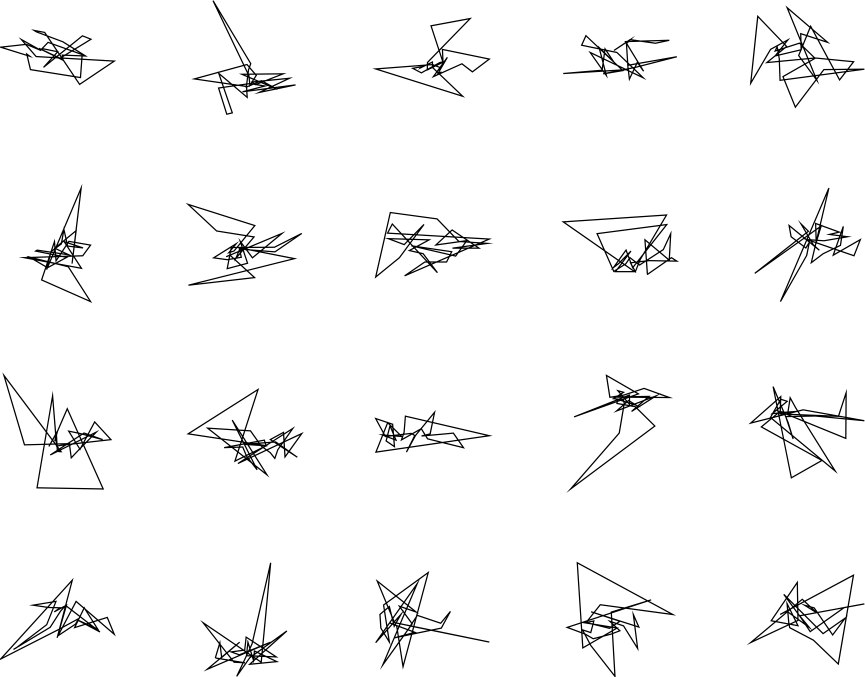
\includegraphics[width=6in]{output/1.models/comparison_gaussians/comparison_gaussians_gaussians_.png}
\subsection{Variance decreased}
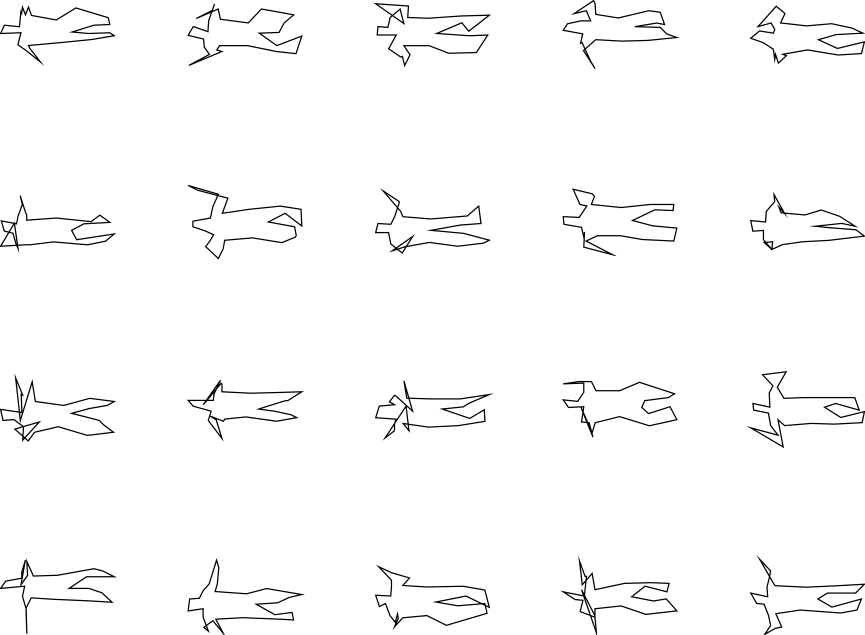
\includegraphics[width=6in]{output/1.models/comparison_gaussians/comparison_gaussians_gaussians_decvar_.png}
\subsection{Variance set to zero}
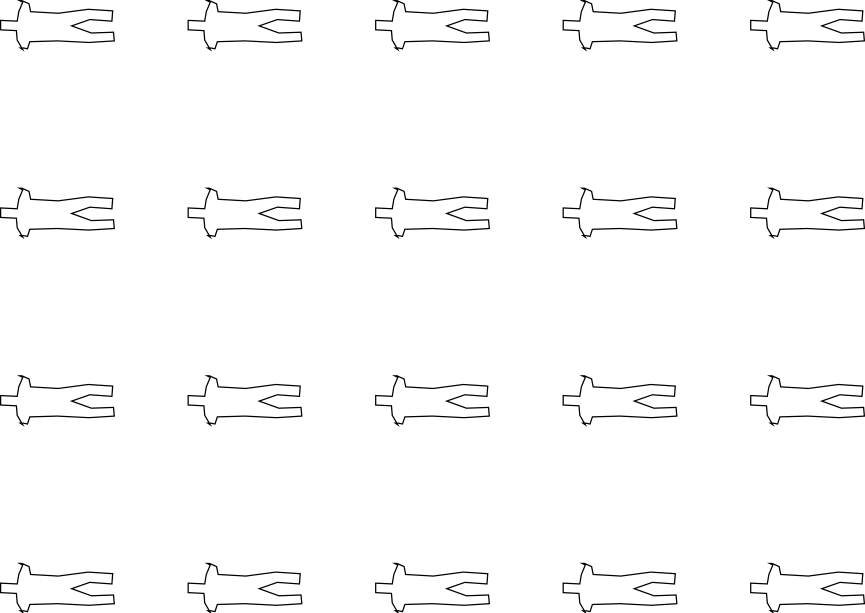
\includegraphics[width=6in]{output/1.models/comparison_gaussians/comparison_gaussians_gaussians_novar_.png}


\section{Independent Nonparametric Distributions}

This model also generates completely nonsensical curves.

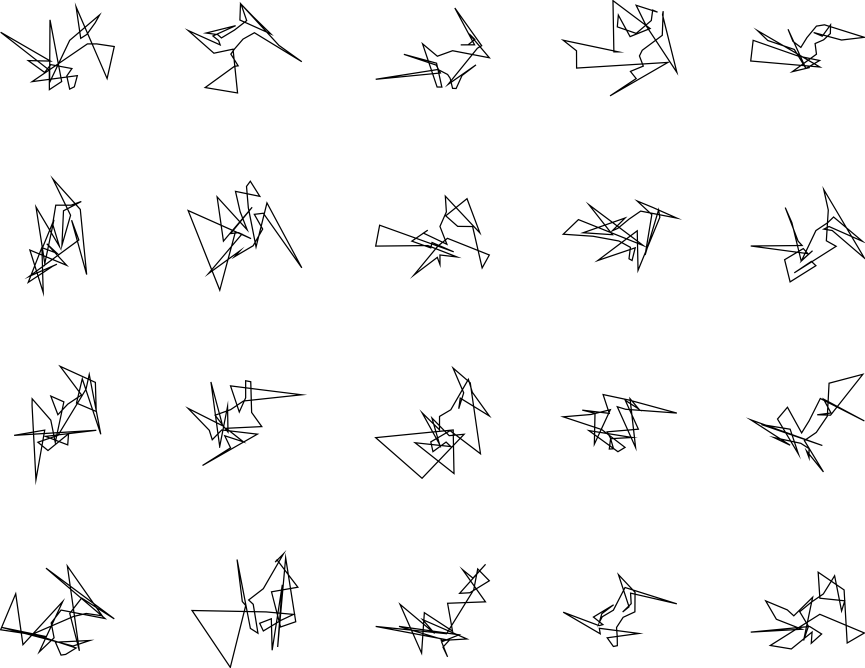
\includegraphics[width=6in]{output/1.models/comparison_parzen/comparison_parzen_parzen_.png}


\chapter{Parameter Learning}

\section{Setup for Learning Experiments}

For each experiment in this section, we build a grammar from the
example curve, train it on the training curves, and then evaluate it
by computing the cross-entropy on the validation curves. 

For all but one of the experiments, we repeat the experiment with
three different starting structures, which are shown below as
decompositions of the example curve.

Unless otherwise noted, these experiments use Watson distributions and
a $Gamma(\sigma=10^6, \overline{\kappa}=1000)$ prior on the
concentration of the Watson distributions.

\subsection{Example Curve}


\includegraphics[width=1in]{output/3.learning/learning_setup/learning_setup_examples_.png}
\subsection{Training Curves}

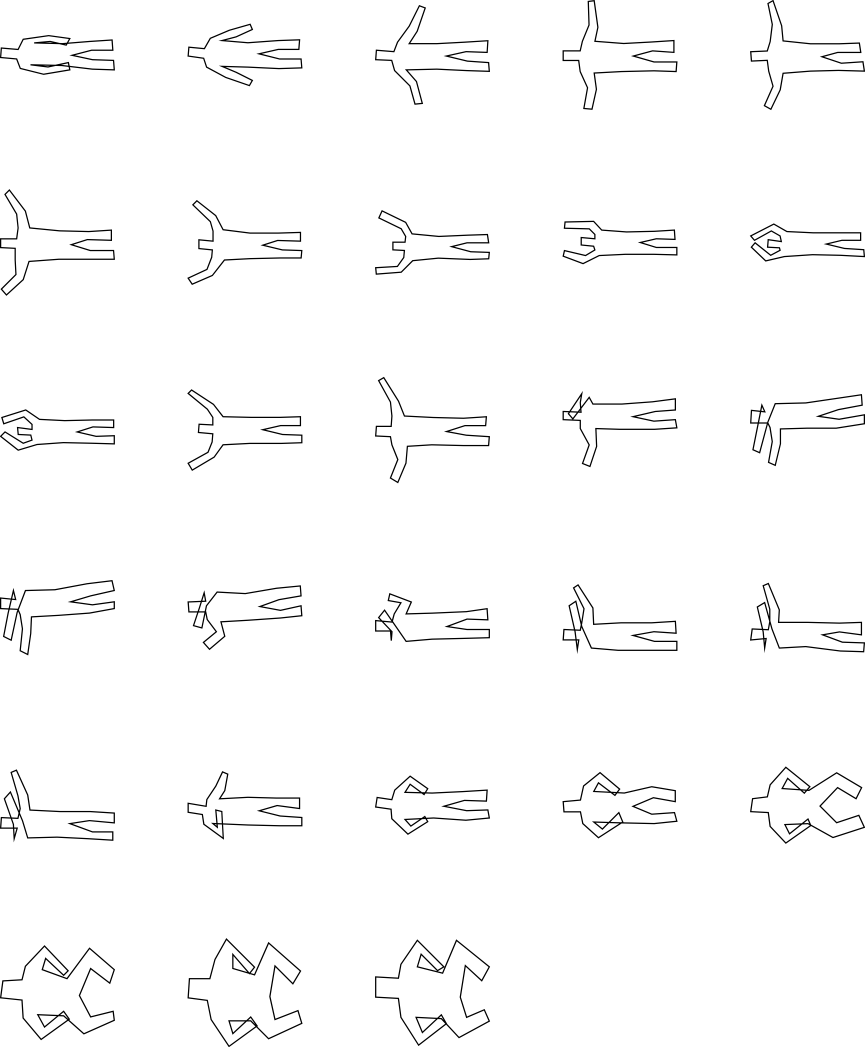
\includegraphics[width=6in]{output/3.learning/learning_setup/learning_setup_training_.png}
\subsection{Validation Curves}

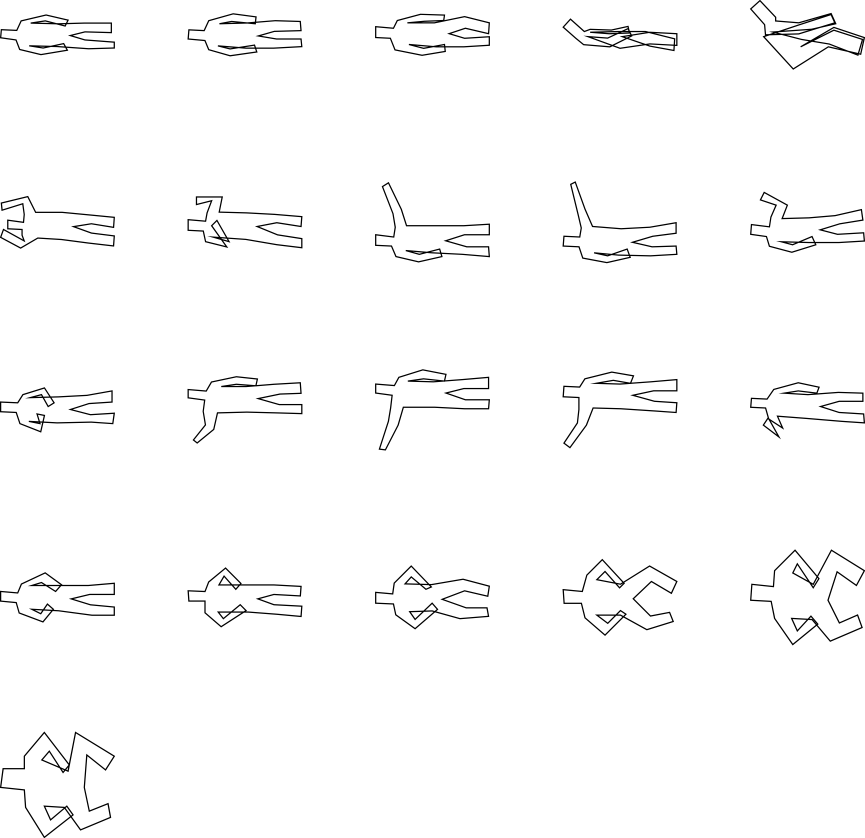
\includegraphics[width=6in]{output/3.learning/learning_setup/learning_setup_validation_.png}
\subsection{Structure \#1}

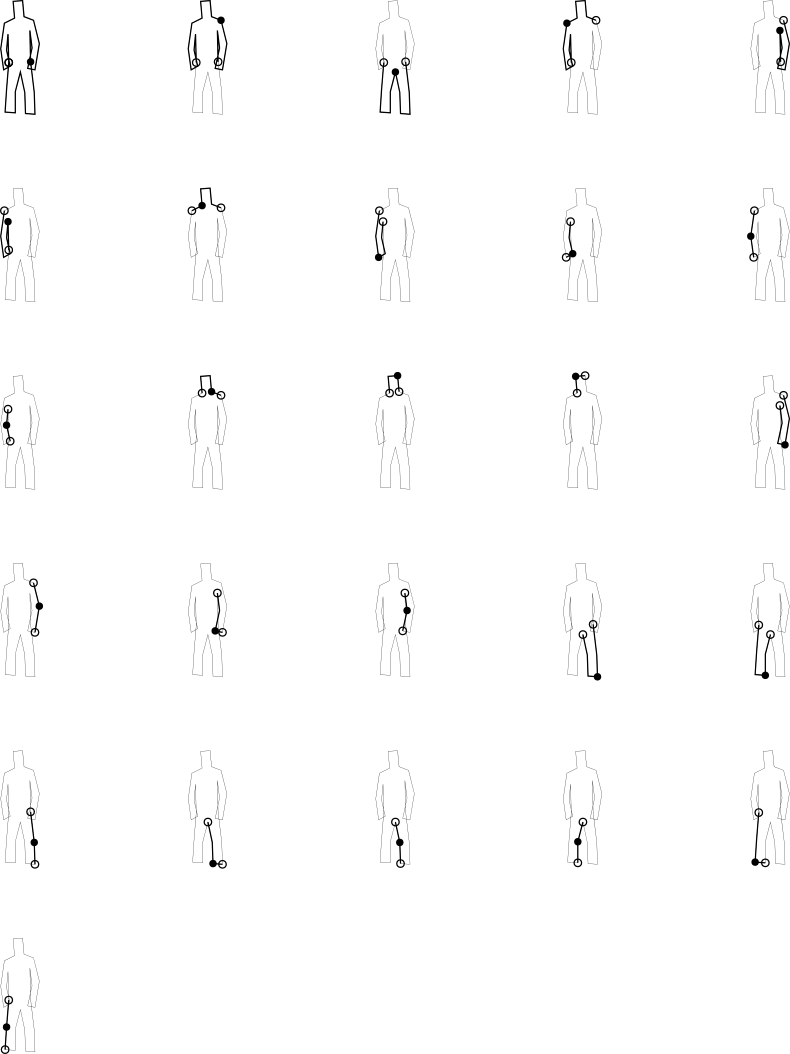
\includegraphics[width=6in]{output/3.learning/learning_setup/learning_setup_sdf0_.png}
\subsection{Structure \#2}

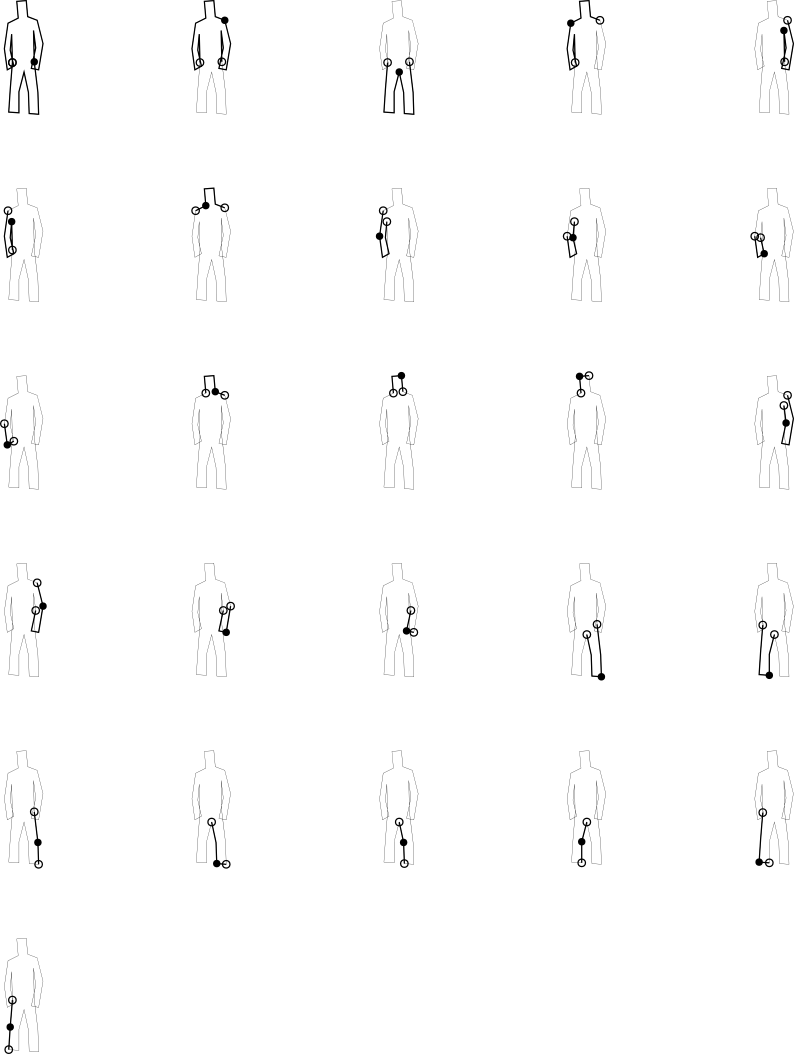
\includegraphics[width=6in]{output/3.learning/learning_setup/learning_setup_sdf1_.png}
\subsection{Structure \#3}

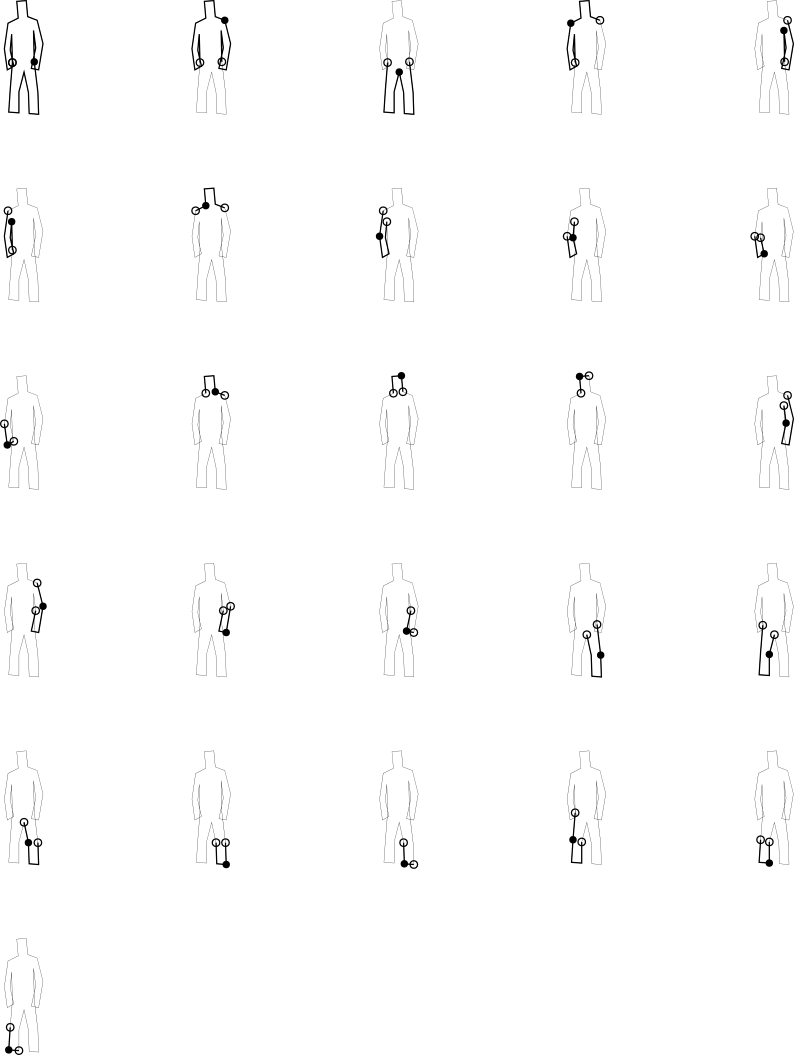
\includegraphics[width=6in]{output/3.learning/learning_setup/learning_setup_sdf2_.png}


\section{Simple Tuning of hand-built grammar with curves of constant length}

First, we use EM to train an initial grammar that has no choices. Our
grammar is produced from a hand-chosen decomposition. Samples from the
grammar after various numbers of rounds of training are shown
below. Since we are using unimodal midpoint distributions, and our
grammar has no choice, all the samples are slight variations on one
particular mean shape. The mean shape chosen is a very reasonable one,
although the arms are longer than is ideal.

We repeat this grammar three times with different initial grammatical
structures, to show how the performance of the algorithm depends on
our initial structure. We also show the log-likelihoods of the data
after each round of training in the table below.

\begin{table}\begin{tabular}{|l|l|l|}
\hline
2792669.441040&2858598.795549&3186255.881673\\
21679.145584&14944.299535&15952.025953\\
21679.145584&14944.299535&15952.025953\\
21679.145584&14944.299535&15952.025953\\
21679.145584&14944.299535&15952.025953\\
21679.145584&14944.299535&15952.025953\\
21679.145584&14944.299535&15952.025953\\
21679.145584&14944.299535&15952.025953\\
21679.145584&14944.299535&15952.025953\\
21679.145584&14944.299535&15952.025953\\
21679.145584&14944.299535&15952.025953\\
21679.145584&14944.299535&15952.025953\\
21679.145584&14944.299535&15952.025953\\
21679.145584&14944.299535&15952.025953\\
21679.145584&14944.299535&15952.025953\\
21679.145584&14944.299535&15952.025953\\
21679.145584&14944.299535&15952.025953\\
21679.145584&14944.299535&15952.025953\\
21679.145584&14944.299535&15952.025953\\
21679.145584&14944.299535&15952.025953\\
21679.145584&14944.299535&15952.025953\\
21679.145584&14944.299535&15952.025953\\
21679.145584&14944.299535&15952.025953\\
21679.145584&14944.299535&15952.025953\\
21679.145584&14944.299535&15952.025953\\
21679.145584&14944.299535&15952.025953\\
21679.145584&14944.299535&15952.025953\\
21679.145584&14944.299535&15952.025953\\
21679.145584&14944.299535&15952.025953\\
21679.145584&14944.299535&15952.025953\\
21679.145584&14944.299535&15952.025953\\
\hline
\end{tabular}\caption{
  Cross-entropy scores across iterations. Each column represents a different starting structure.}\end{table}

\subsection{Simple Tuning with SDF 1}

\subsubsection{After 0 iterations}

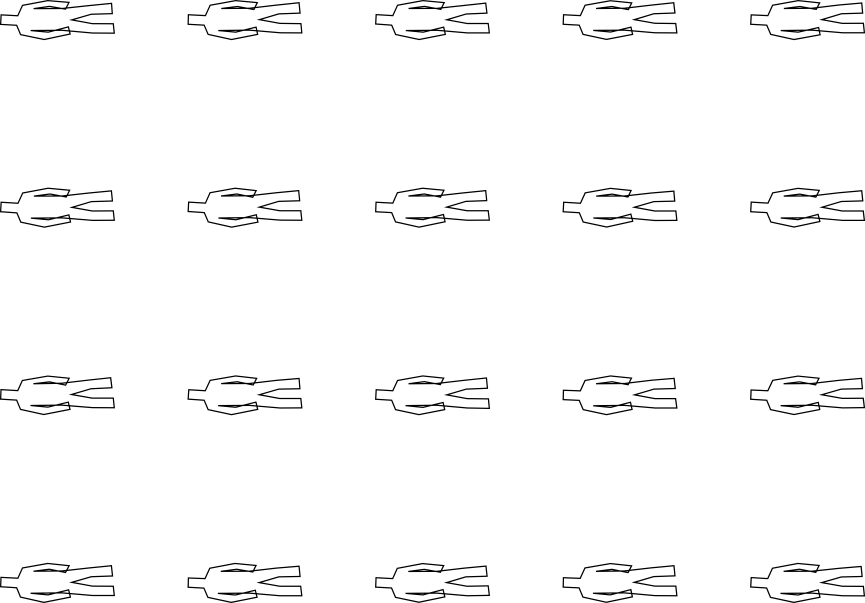
\includegraphics[width=6in]{output/3.learning/simple_tuning/simple_tuning_iter0_.png}
\subsubsection{After 10 iterations}

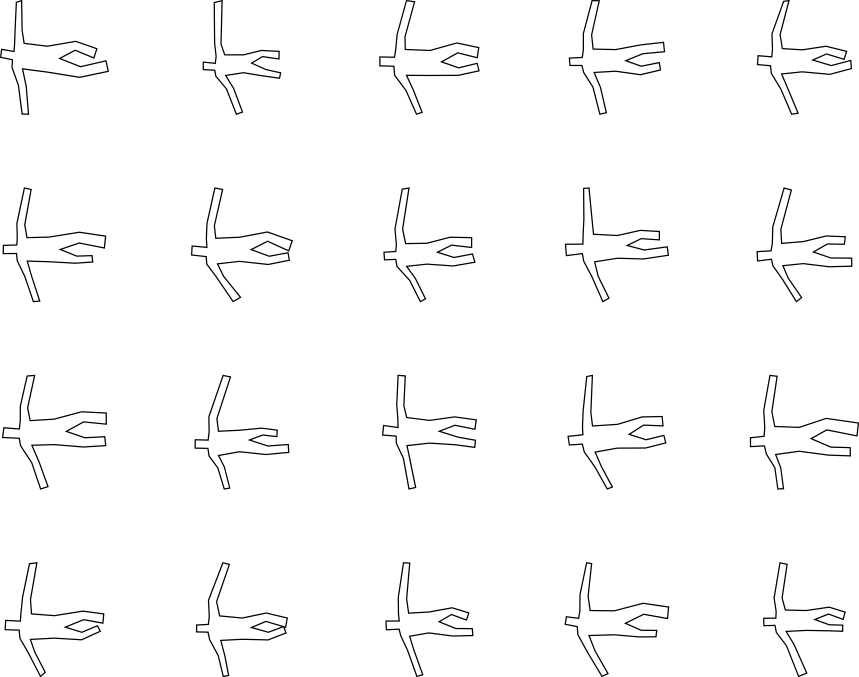
\includegraphics[width=6in]{output/3.learning/simple_tuning/simple_tuning_iter10_.png}
\subsubsection{After 20 iterations}

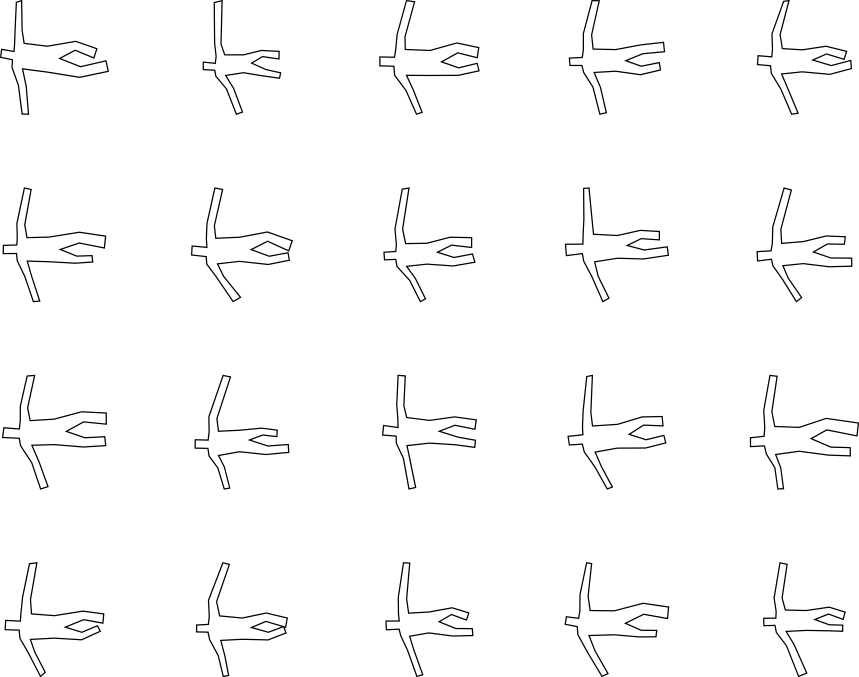
\includegraphics[width=6in]{output/3.learning/simple_tuning/simple_tuning_iter20_.png}
\subsubsection{After 30 iterations}

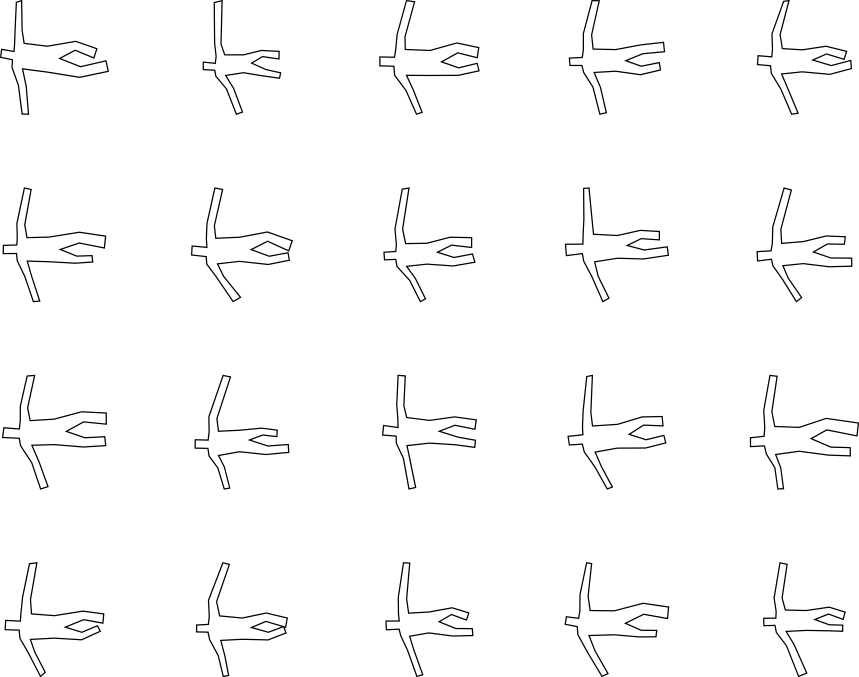
\includegraphics[width=6in]{output/3.learning/simple_tuning/simple_tuning_iter30_.png}
\subsection{Simple Tuning with SDF 2}

\subsubsection{After 0 iterations}

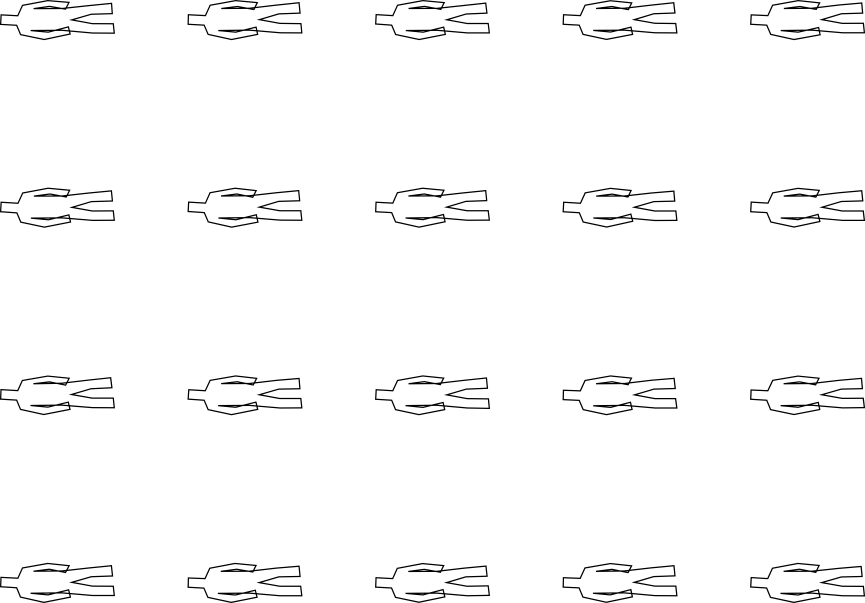
\includegraphics[width=6in]{output/3.learning/simple_tuning/simple_tuning_iter0_.png}
\subsubsection{After 10 iterations}

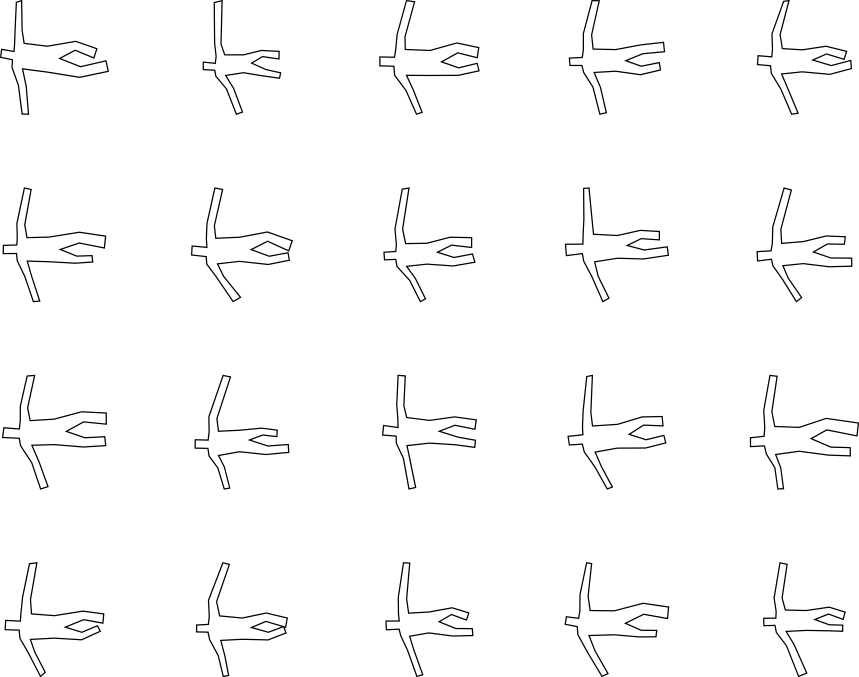
\includegraphics[width=6in]{output/3.learning/simple_tuning/simple_tuning_iter10_.png}
\subsubsection{After 20 iterations}

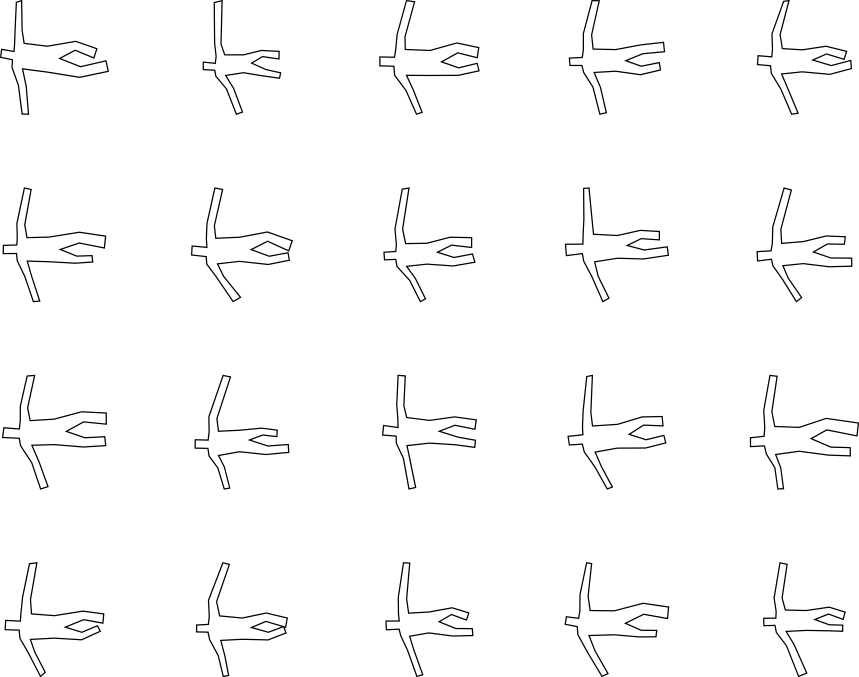
\includegraphics[width=6in]{output/3.learning/simple_tuning/simple_tuning_iter20_.png}
\subsubsection{After 30 iterations}

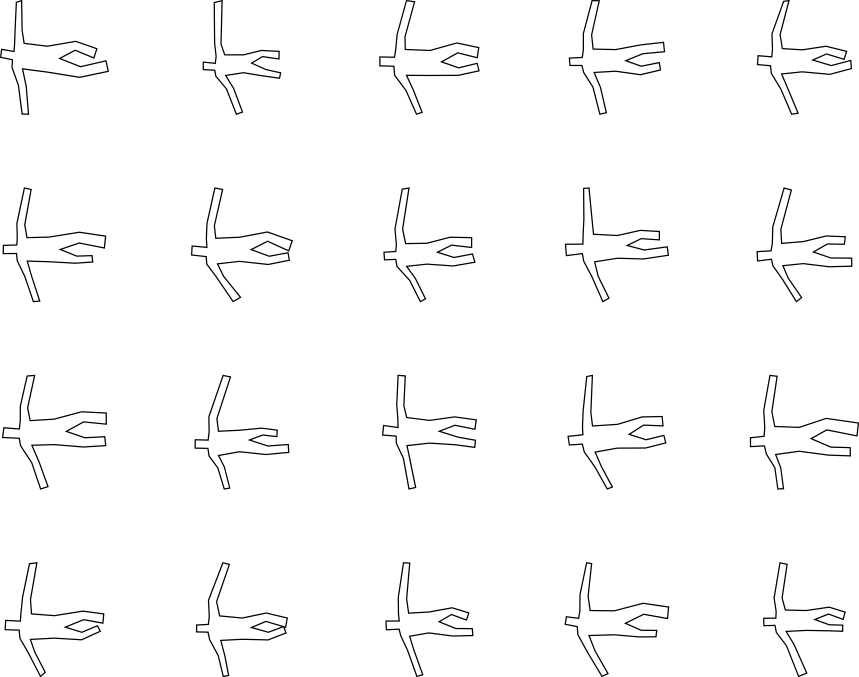
\includegraphics[width=6in]{output/3.learning/simple_tuning/simple_tuning_iter30_.png}
\subsection{Simple Tuning with SDF 3}

\subsubsection{After 0 iterations}

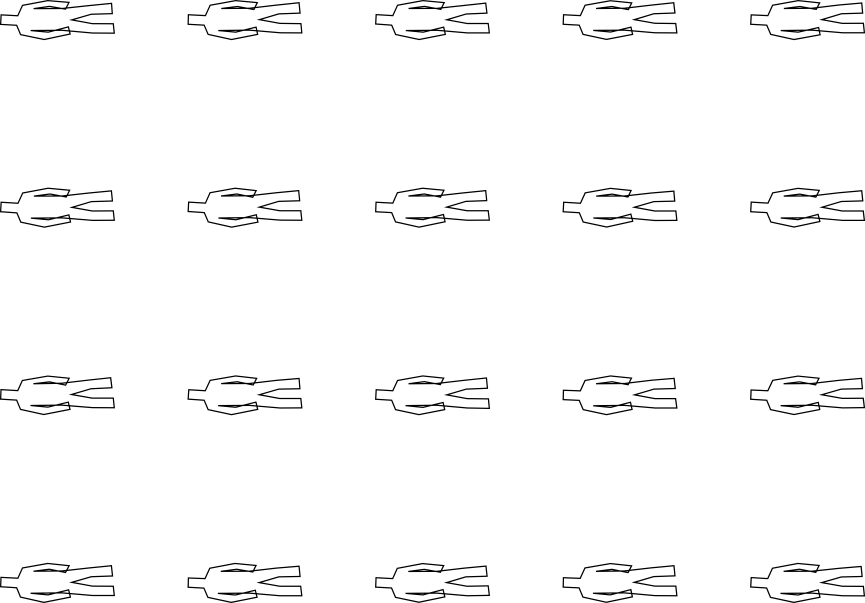
\includegraphics[width=6in]{output/3.learning/simple_tuning/simple_tuning_iter0_.png}
\subsubsection{After 10 iterations}

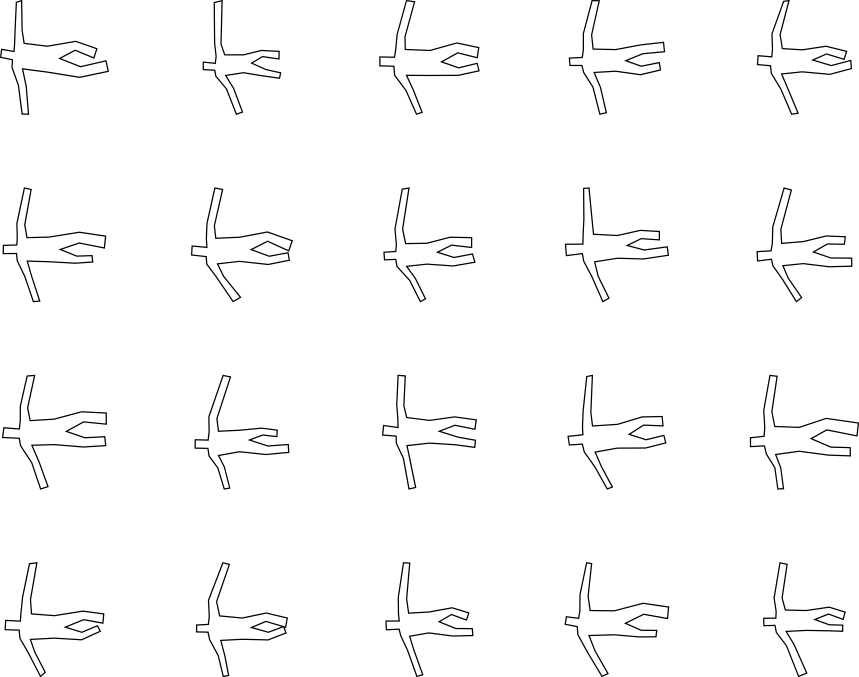
\includegraphics[width=6in]{output/3.learning/simple_tuning/simple_tuning_iter10_.png}
\subsubsection{After 20 iterations}

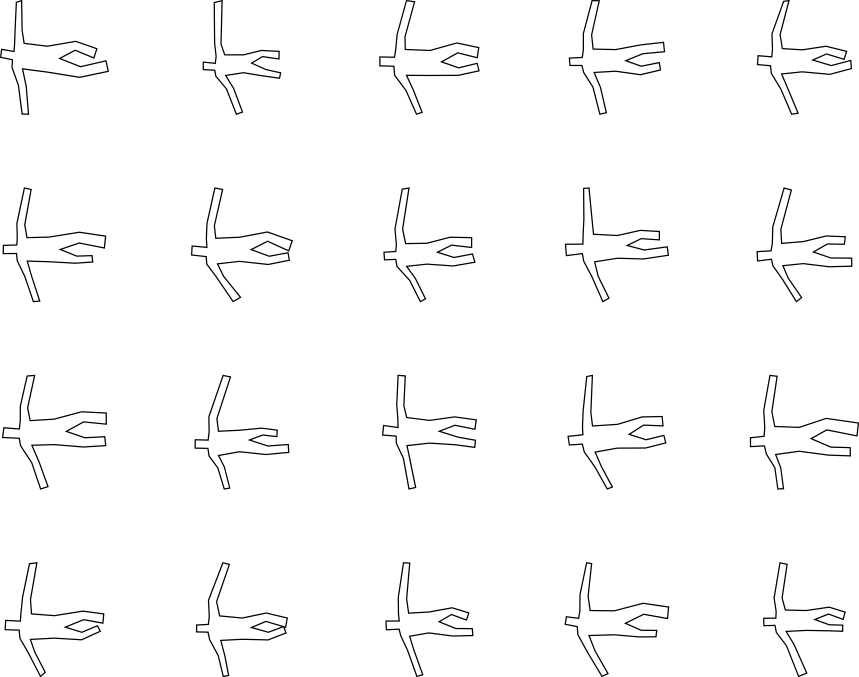
\includegraphics[width=6in]{output/3.learning/simple_tuning/simple_tuning_iter20_.png}
\subsubsection{After 30 iterations}

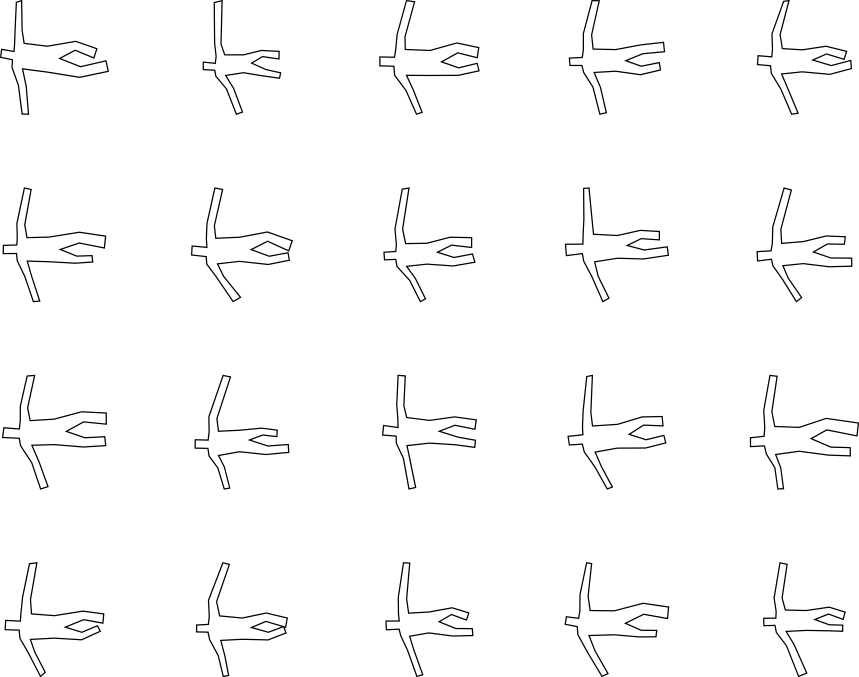
\includegraphics[width=6in]{output/3.learning/simple_tuning/simple_tuning_iter30_.png}


\section{Experimenting with different priors over concentration}

Here we are using Watson distributions and a $Gamma(\sigma,
\overline{\kappa}=100)$ prior on the concentration of the Watson
distributions, for $\sigma=1, 1000, 10^6$.

\begin{table}\begin{tabular}{|l|l|l|l|}
\hline
1&1000&1000000\\
\hline\\
2858598.795549&2858598.795549&2858598.795549\\
235.329827&688.733064&851.271307\\
235.329827&688.733064&851.271307\\
235.329827&688.733064&851.271307\\
235.329827&688.733064&851.271307\\
235.329827&688.733064&851.271307\\
235.329827&688.733064&851.271307\\
235.329827&688.733064&851.271307\\
235.329827&688.733064&851.271307\\
235.329827&688.733064&851.271307\\
235.329827&688.733064&851.271307\\
235.329827&688.733064&851.271307\\
235.329827&688.733064&851.271307\\
235.329827&688.733064&851.271307\\
235.329827&688.733064&851.271307\\
235.329827&688.733064&851.271307\\
235.329827&688.733064&851.271307\\
235.329827&688.733064&851.271307\\
235.329827&688.733064&851.271307\\
235.329827&688.733064&851.271307\\
235.329827&688.733064&851.271307\\
235.329827&688.733064&851.271307\\
235.329827&688.733064&851.271307\\
235.329827&688.733064&851.271307\\
235.329827&688.733064&851.271307\\
235.329827&688.733064&851.271307\\
235.329827&688.733064&851.271307\\
235.329827&688.733064&851.271307\\
235.329827&688.733064&851.271307\\
235.329827&688.733064&851.271307\\
\hline
\end{tabular}\caption{
Cross-entropy scores across iterations. Each column represents a different weight given to the prior over concentrations.}\end{table}

\subsection{Tuning with Different Priors on Concentration with $\sigma=1$}

\subsubsection{After 0 iterations}

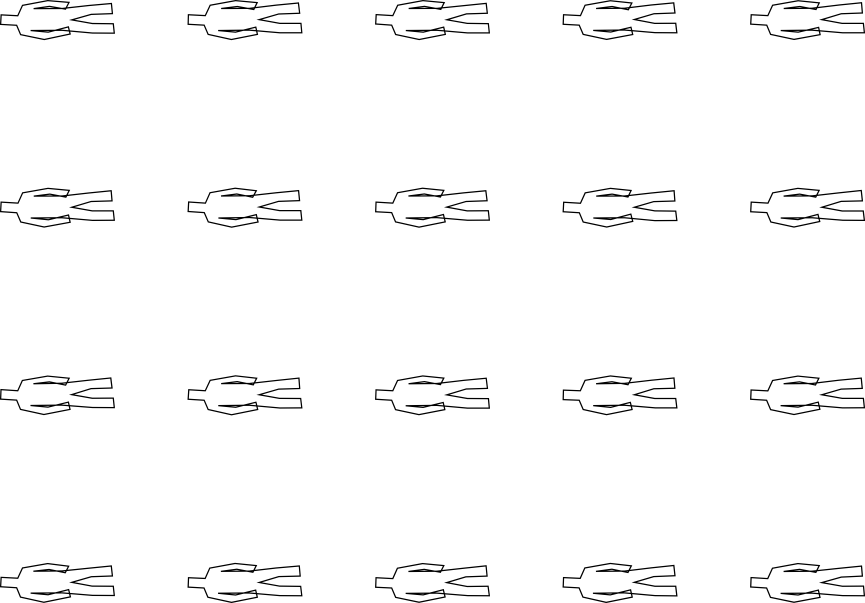
\includegraphics[width=6in]{output/3.learning/concentration/concentration_psw1_iter0_.png}
\subsubsection{After 10 iterations}

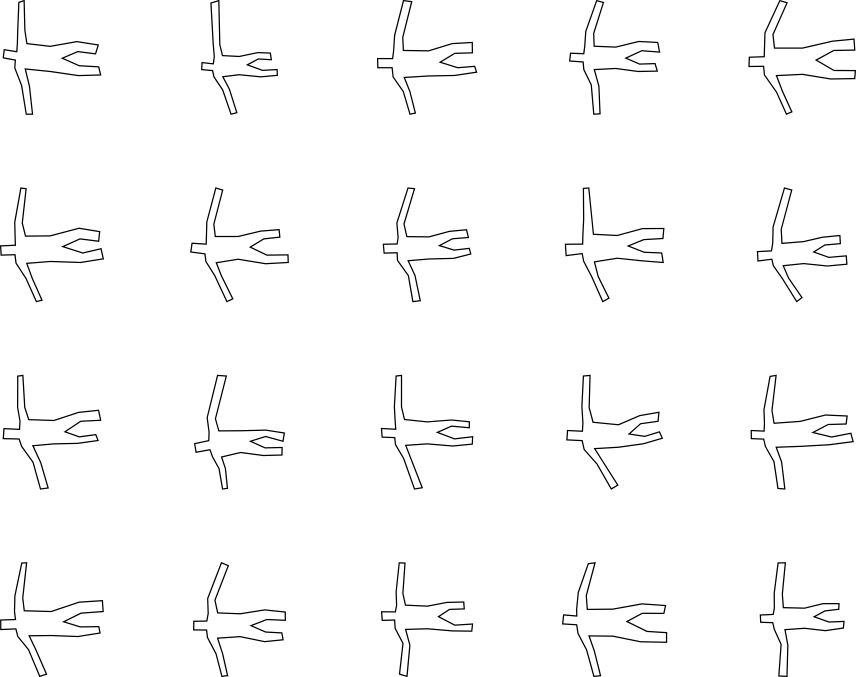
\includegraphics[width=6in]{output/3.learning/concentration/concentration_psw1_iter10_.png}
\subsubsection{After 20 iterations}

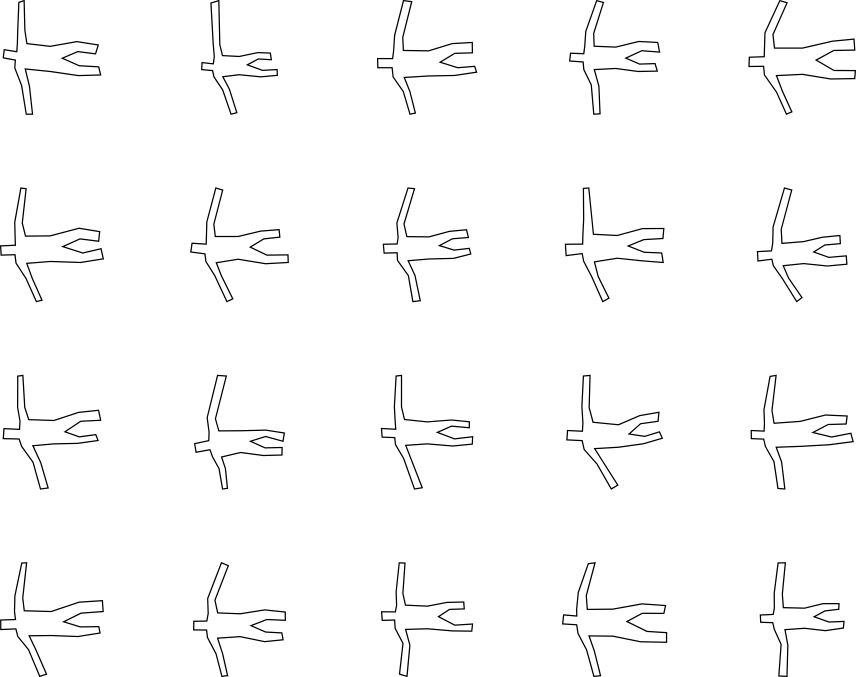
\includegraphics[width=6in]{output/3.learning/concentration/concentration_psw1_iter20_.png}
\subsubsection{After 30 iterations}

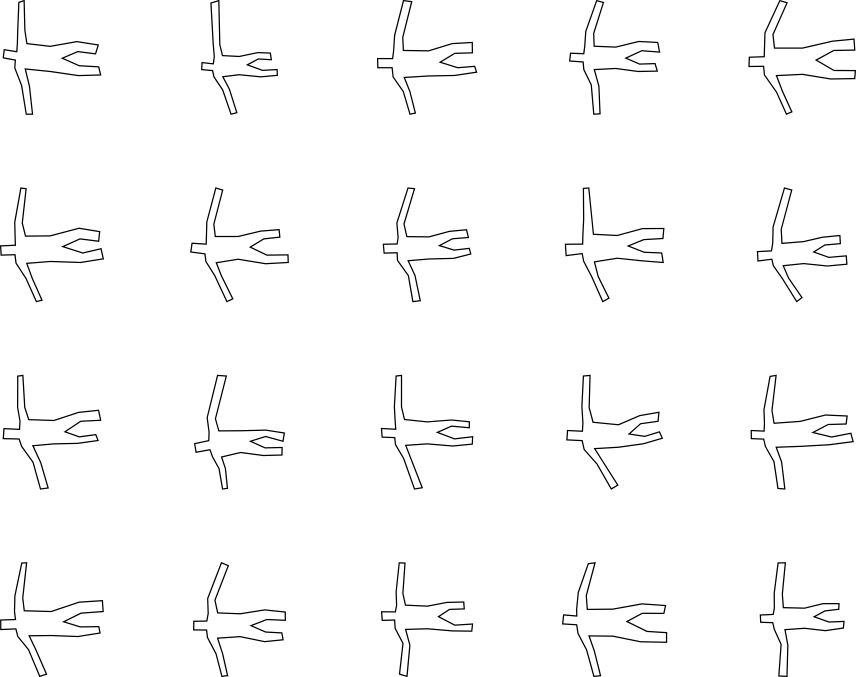
\includegraphics[width=6in]{output/3.learning/concentration/concentration_psw1_iter30_.png}
\subsection{Tuning with Different Priors on Concentration with $\sigma=1000$}

\subsubsection{After 0 iterations}

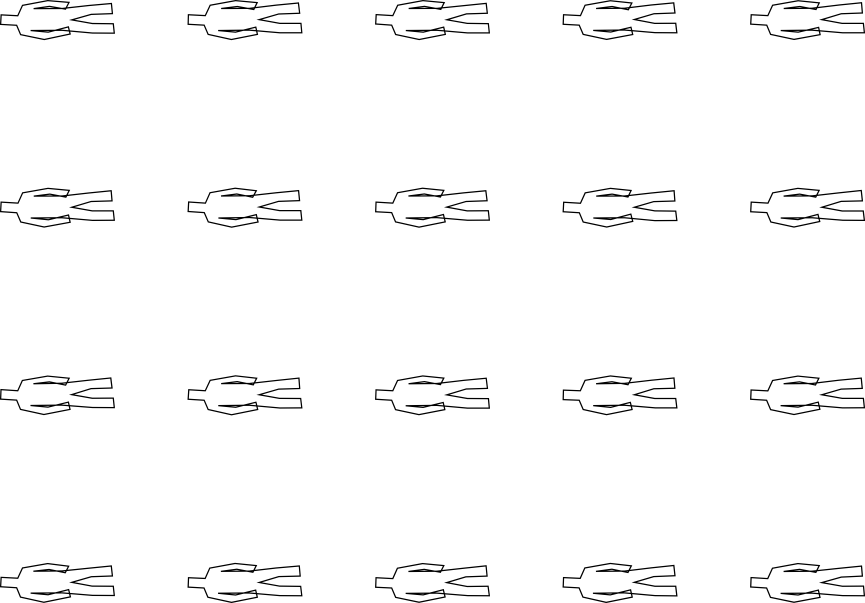
\includegraphics[width=6in]{output/3.learning/concentration/concentration_psw1000_iter0_.png}
\subsubsection{After 10 iterations}

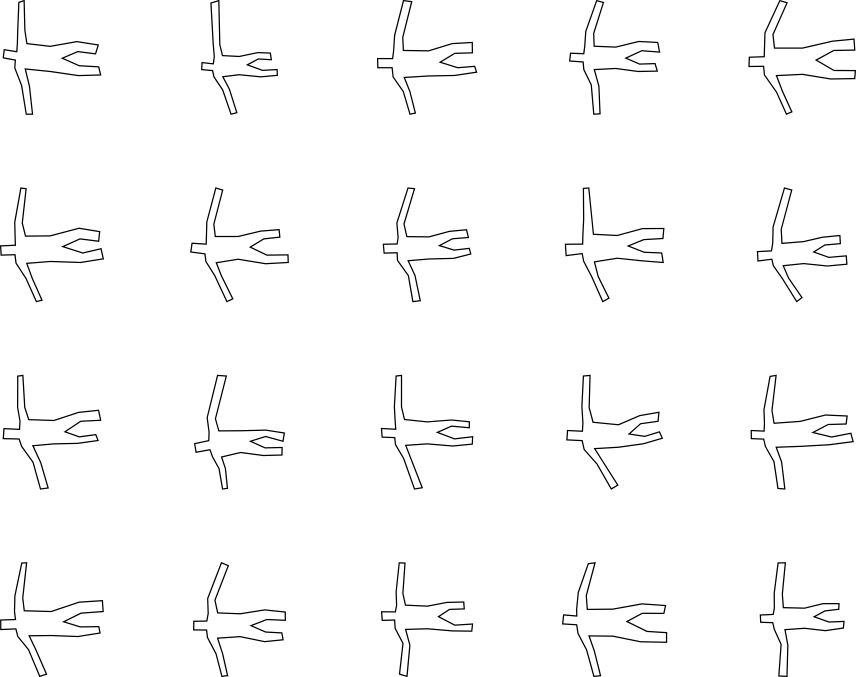
\includegraphics[width=6in]{output/3.learning/concentration/concentration_psw1000_iter10_.png}
\subsubsection{After 20 iterations}

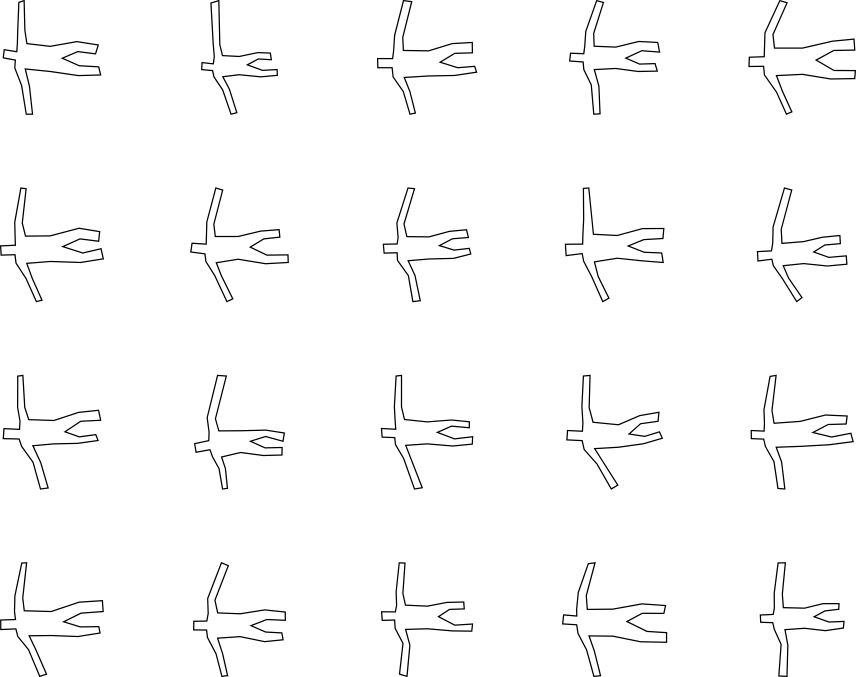
\includegraphics[width=6in]{output/3.learning/concentration/concentration_psw1000_iter20_.png}
\subsubsection{After 30 iterations}

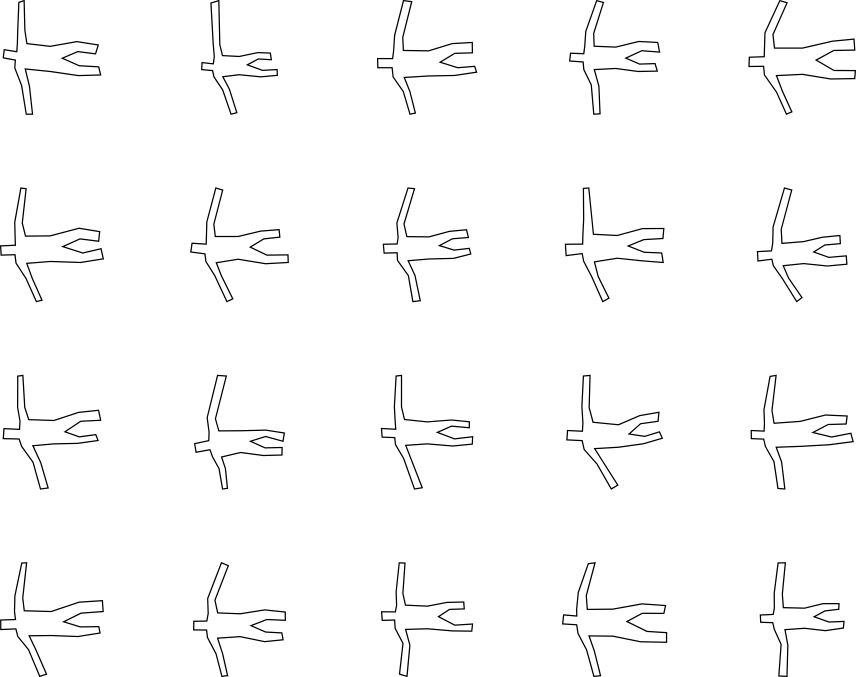
\includegraphics[width=6in]{output/3.learning/concentration/concentration_psw1000_iter30_.png}
\subsection{Tuning with Different Priors on Concentration with $\sigma=1000000$}

\subsubsection{After 0 iterations}

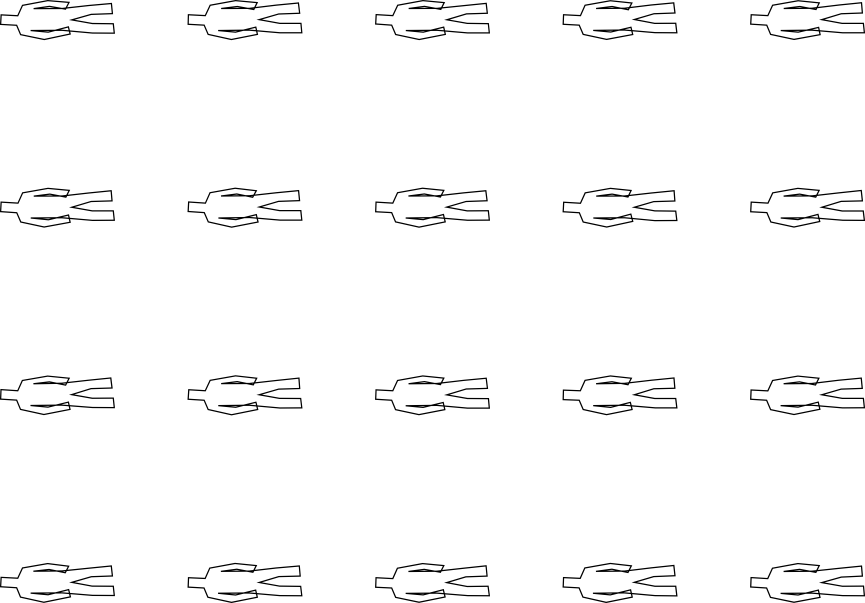
\includegraphics[width=6in]{output/3.learning/concentration/concentration_psw1000000_iter0_.png}
\subsubsection{After 10 iterations}

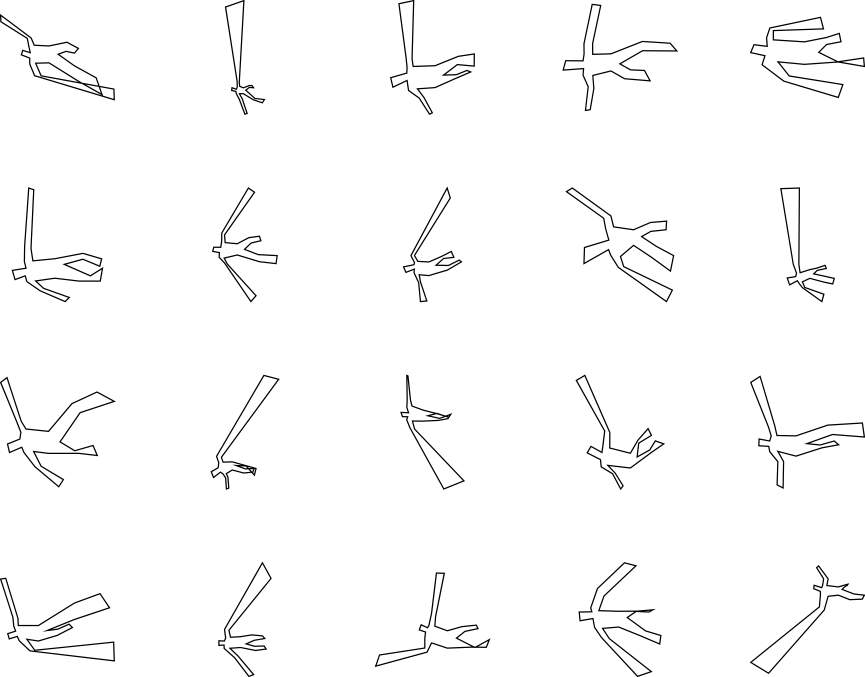
\includegraphics[width=6in]{output/3.learning/concentration/concentration_psw1000000_iter10_.png}
\subsubsection{After 20 iterations}

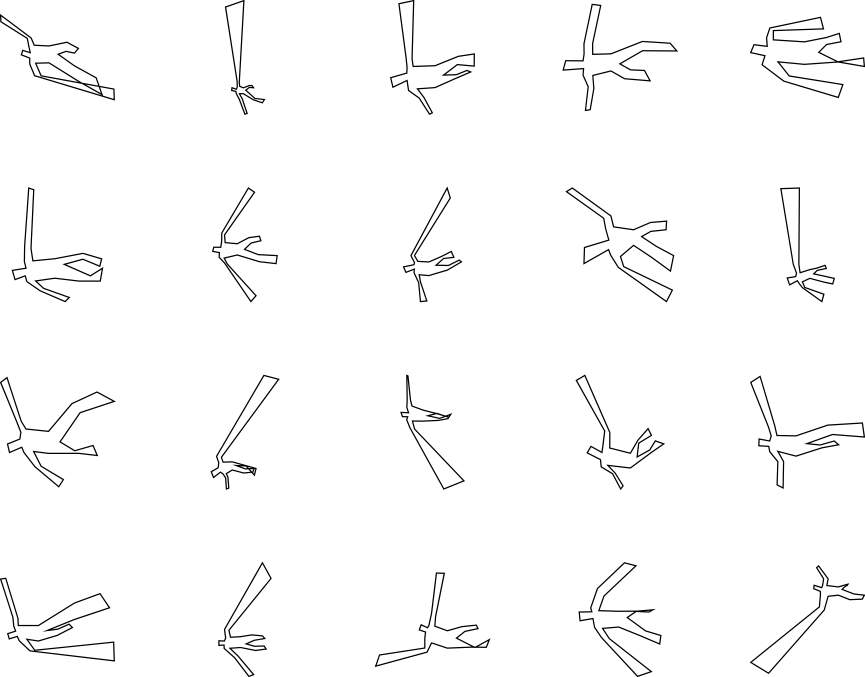
\includegraphics[width=6in]{output/3.learning/concentration/concentration_psw1000000_iter20_.png}
\subsubsection{After 30 iterations}

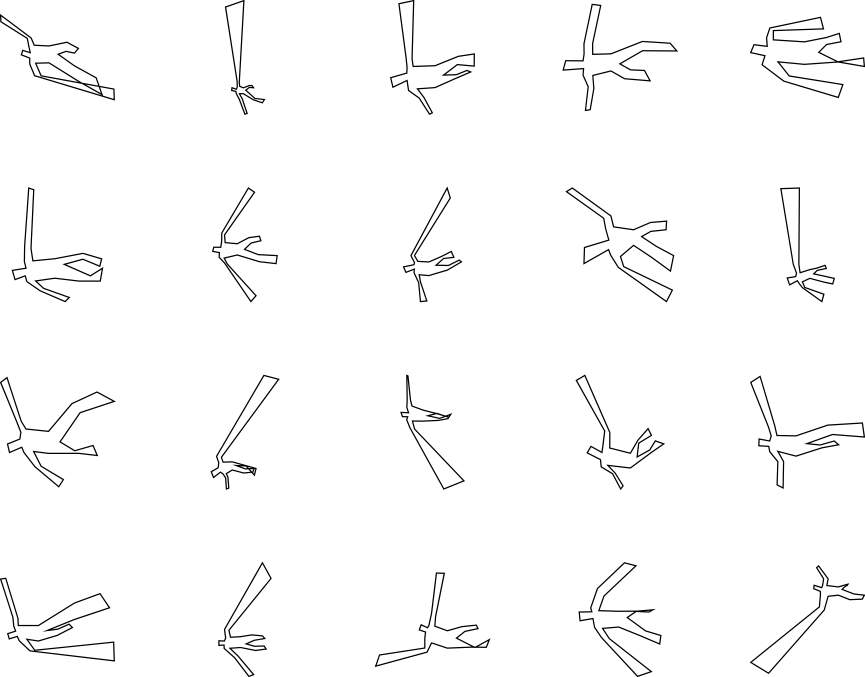
\includegraphics[width=6in]{output/3.learning/concentration/concentration_psw1000000_iter30_.png}


\section{Tuning with multiple midpoints, and curves of constant length}

In the next experiment, we enrich the grammar by adding in several
copies (in this case, five) of each rule, with jittered midpoints. (If
we used the same midpoint for each copy of the rule, parses could use
the rules interchangeably, and EM would never break this symmetry.)
Below, we show samples from the grammar after various numbers of
rounds of training. The samples show significantly more variation than
in the previous experiment, but they also include many ill-formed and
unlikely shapes. This is because the grammar cannot model correlations
between levels, so that e.g., it cannot pick the location of the elbow
based on the location of the hand, which means that the arm is often
ill-formed and self-intersecting.

We repeat this grammar three times with different initial grammatical
structures, to show how the performance of the algorithm depends on
our initial structure. We also show the log-likelihoods of the data
after each round of training in the table below.

\begin{table}\begin{tabular}{|l|l|l|}
\hline
2766135.995375&2831786.003535&3155994.673769\\
8648.267302&7066.649020&7713.649908\\
7773.555218&6157.197659&7332.472119\\
7774.914509&5883.522840&7059.798905\\
7726.281465&5870.701485&7015.282988\\
7686.102388&5889.921155&7010.640463\\
7655.057598&5892.507871&6980.337046\\
7620.810411&5874.575675&6957.516851\\
7609.881760&5867.341009&6954.901441\\
7585.652506&5858.522579&6950.759990\\
7574.061702&5845.430605&6945.285768\\
7560.360288&5829.025699&6941.703432\\
7557.002890&5821.945800&6936.133052\\
7558.127804&5825.647714&6938.649345\\
7565.042698&5829.093529&6941.563464\\
7571.452354&5831.593728&6943.697000\\
7575.688781&5833.315355&6944.660214\\
7577.695321&5834.497324&6944.754959\\
7578.739088&5835.318945&6940.330486\\
7579.361056&5835.876676&6935.062410\\
7579.761286&5836.252670&6934.039116\\
7580.030977&5836.509946&6933.744380\\
7580.219010&5836.690326&6933.553635\\
7580.354828&5836.821075&6933.405242\\
7580.457458&5836.920285&6933.284399\\
7580.539423&5836.999949&6933.181858\\
7580.608685&5837.067683&6933.091095\\
7580.669893&5837.127896&6933.007889\\
7580.725401&5837.182776&6932.929834\\
7580.776160&5837.233156&6932.855793\\
7580.822413&5837.279200&6932.785398\\
\hline
\end{tabular}\caption{
  Cross-entropy scores across iterations. Each column represents a different starting structure.}\end{table}

\subsection{Tuning with multiple midpoints with SDF 1}

\subsubsection{After 0 iterations}

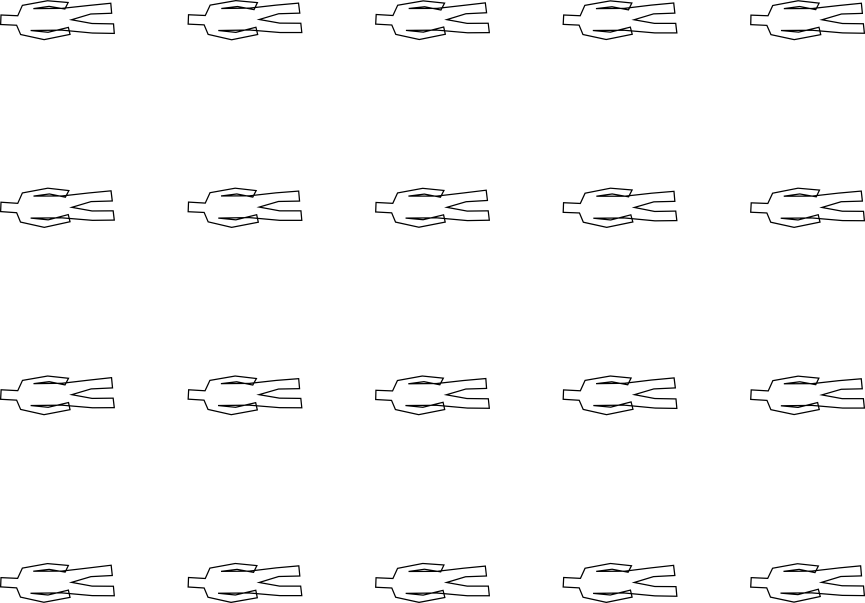
\includegraphics[width=6in]{output/3.learning/multi_tuning/multi_tuning_iter0_.png}
\subsubsection{After 10 iterations}

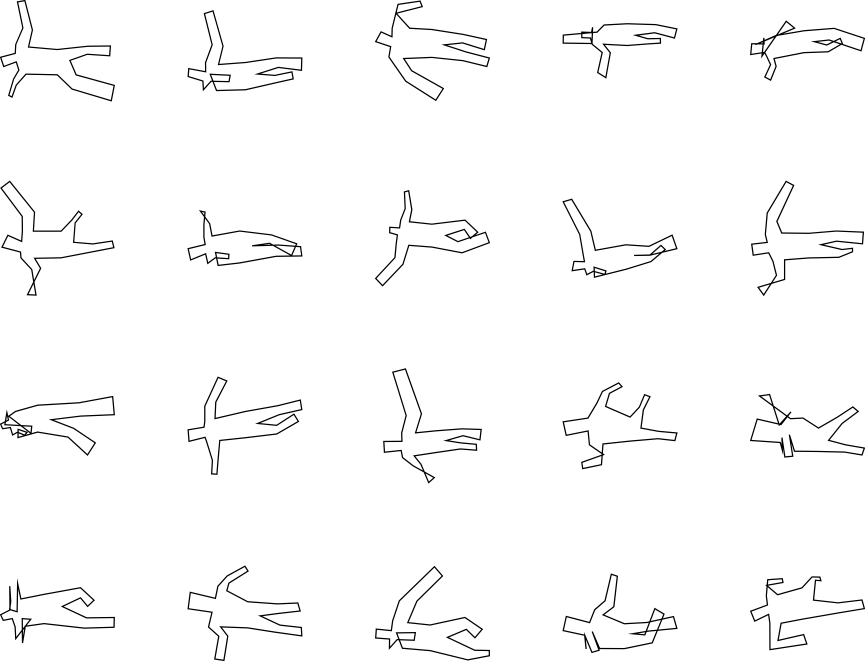
\includegraphics[width=6in]{output/3.learning/multi_tuning/multi_tuning_iter10_.png}
\subsubsection{After 20 iterations}

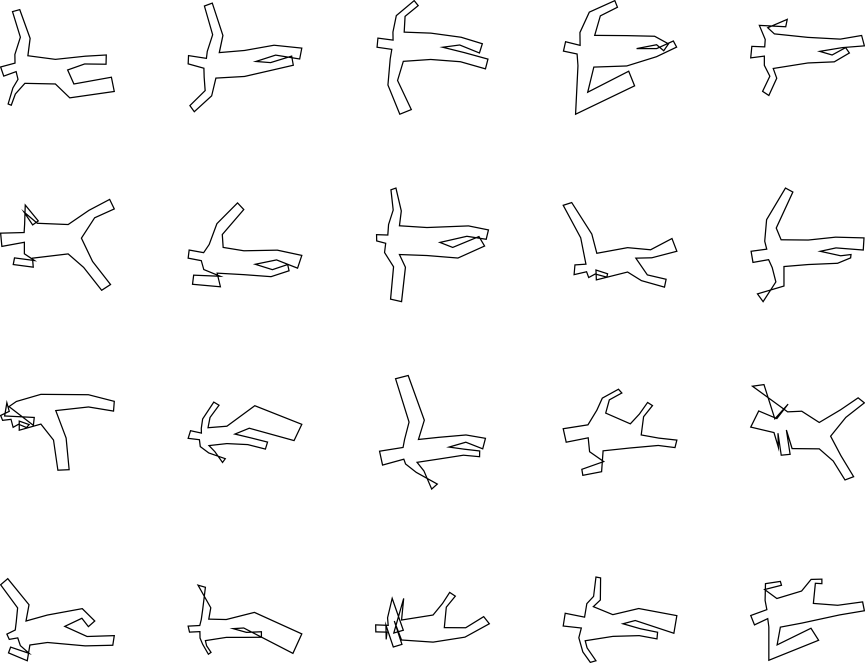
\includegraphics[width=6in]{output/3.learning/multi_tuning/multi_tuning_iter20_.png}
\subsubsection{After 30 iterations}

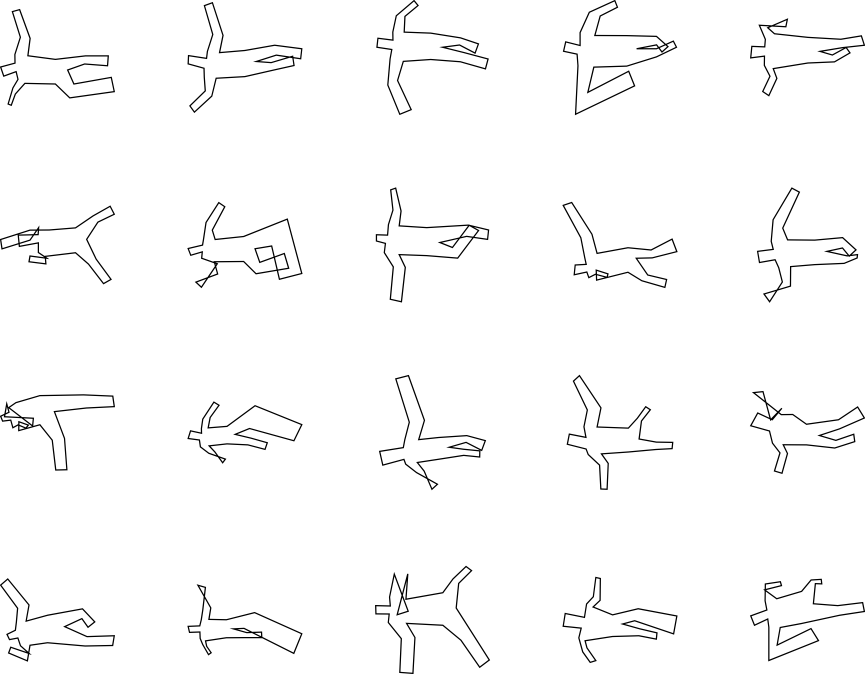
\includegraphics[width=6in]{output/3.learning/multi_tuning/multi_tuning_iter30_.png}
\subsection{Tuning with multiple midpoints with SDF 2}

\subsubsection{After 0 iterations}

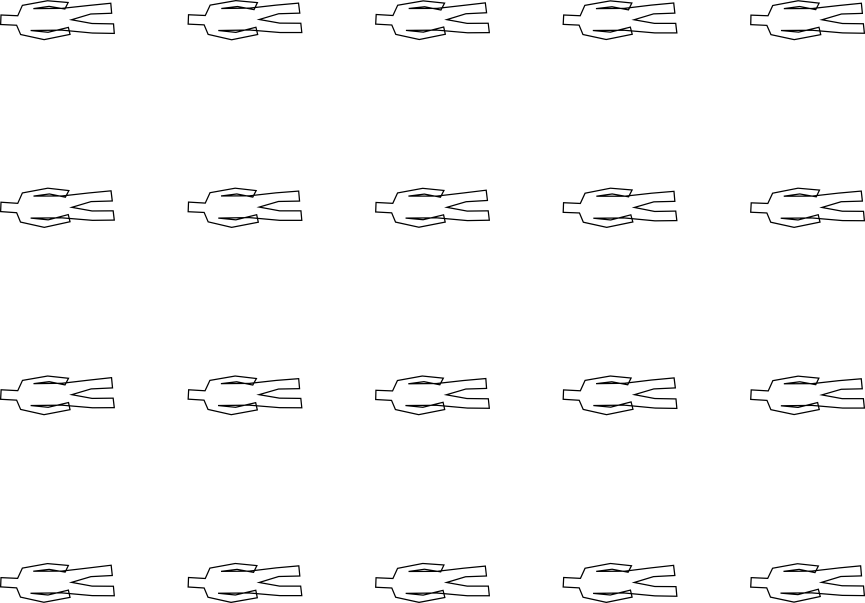
\includegraphics[width=6in]{output/3.learning/multi_tuning/multi_tuning_iter0_.png}
\subsubsection{After 10 iterations}

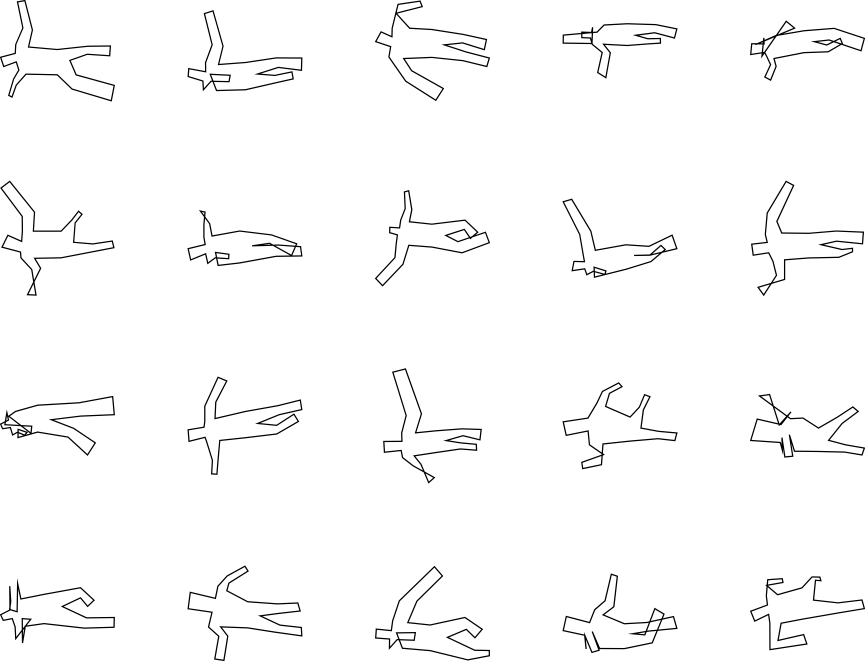
\includegraphics[width=6in]{output/3.learning/multi_tuning/multi_tuning_iter10_.png}
\subsubsection{After 20 iterations}

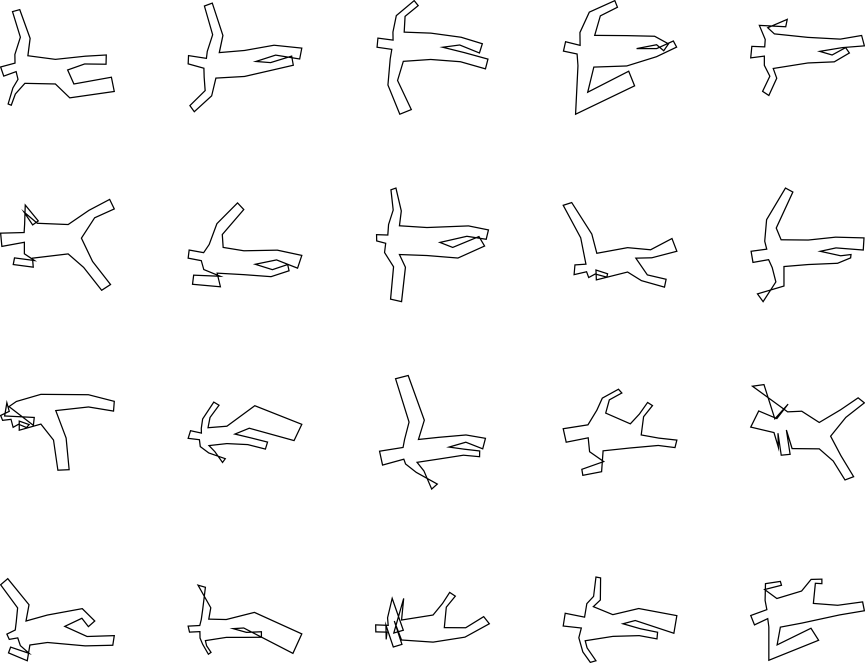
\includegraphics[width=6in]{output/3.learning/multi_tuning/multi_tuning_iter20_.png}
\subsubsection{After 30 iterations}

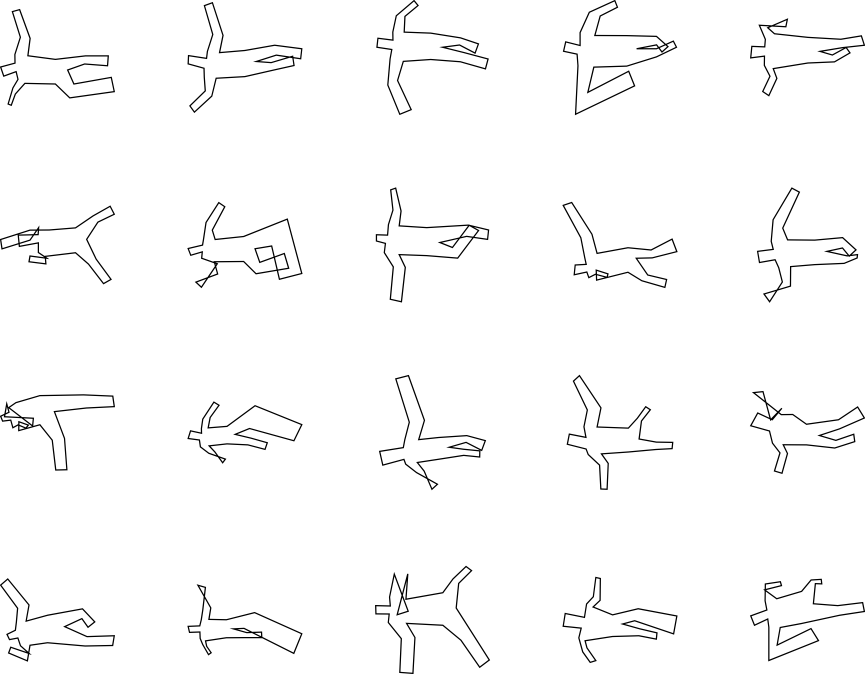
\includegraphics[width=6in]{output/3.learning/multi_tuning/multi_tuning_iter30_.png}
\subsection{Tuning with multiple midpoints with SDF 3}

\subsubsection{After 0 iterations}

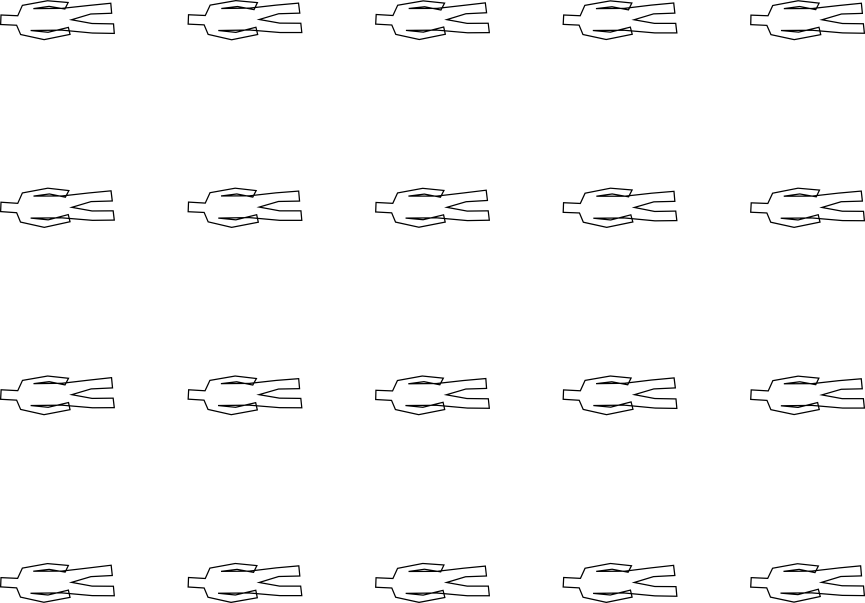
\includegraphics[width=6in]{output/3.learning/multi_tuning/multi_tuning_iter0_.png}
\subsubsection{After 10 iterations}

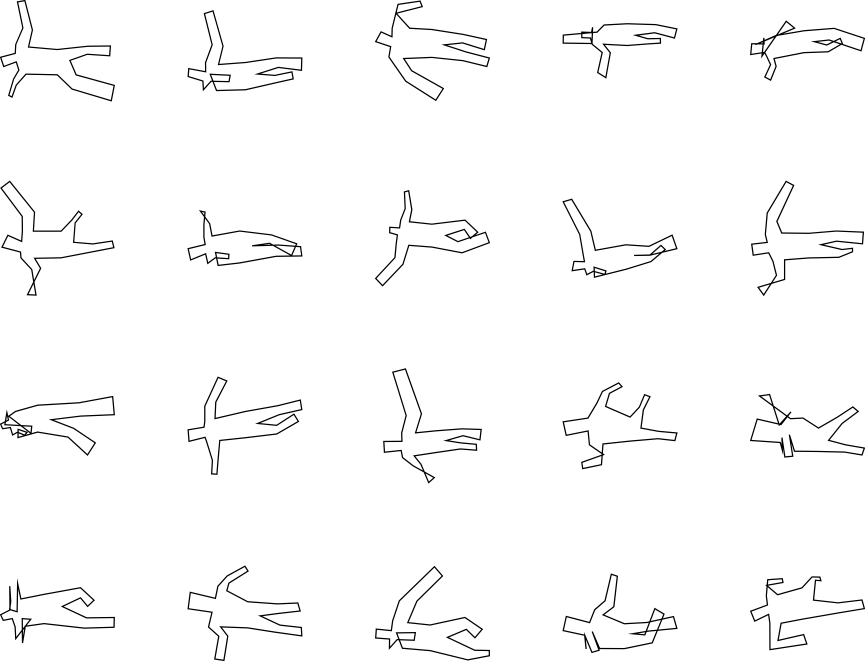
\includegraphics[width=6in]{output/3.learning/multi_tuning/multi_tuning_iter10_.png}
\subsubsection{After 20 iterations}

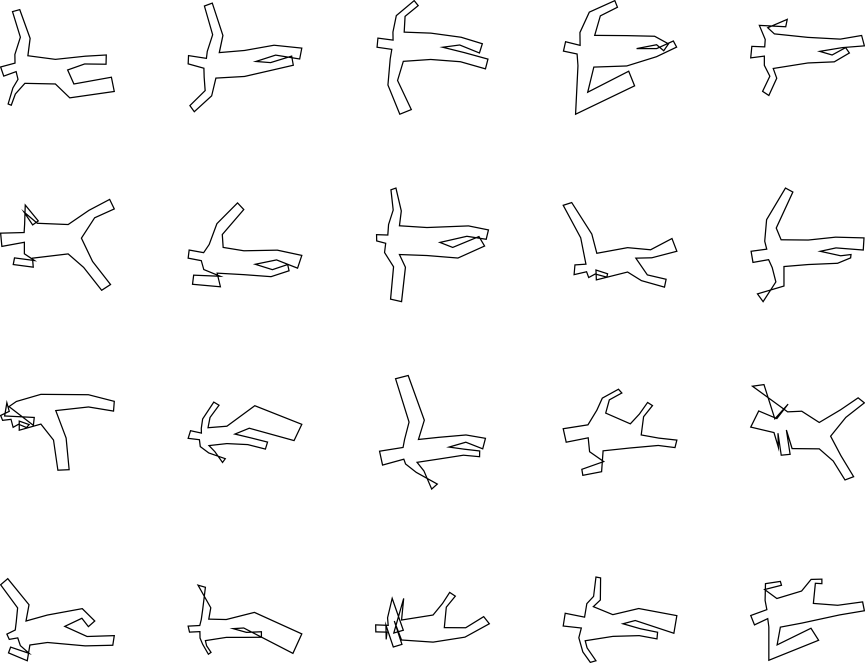
\includegraphics[width=6in]{output/3.learning/multi_tuning/multi_tuning_iter20_.png}
\subsubsection{After 30 iterations}

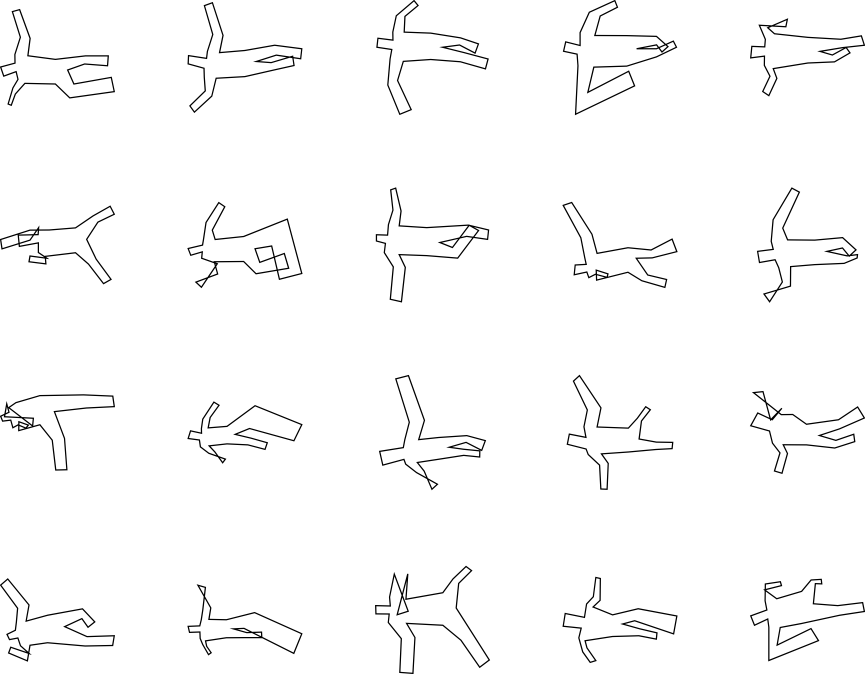
\includegraphics[width=6in]{output/3.learning/multi_tuning/multi_tuning_iter30_.png}


\section{Tuning with multiple midpoints, learning multi-level correlations}

In this experiment, we enrich the grammar by adding in several copies
of each nonterminal, each of which has several copies of the original
rule with jittered midpoints. If our original rule was $X\to YZ$, then
we have five copies each of $X,Y,Z$, and each $X_i$ has five rules of
the form $X_i \to Y_j Z_k$, where $j$ and $k$ are chosen independently
at random.

Below, we show samples from the grammar after various numbers of
rounds of training. The silhouettes look much better than in the
previous experiment. This is because we have learned correlations
between levels, i.e., the choice of rule at a higher level influences
the choice of rule at a lower level.

We repeat this grammar three times with different initial grammatical
structures, to show how the performance of the algorithm depends on
our initial structure. We also show the log-likelihoods of the data
after each round of training in the table below.

\begin{table}\begin{tabular}{|l|l|l|}
\hline
2749190.944197&2816958.726886&3142344.074439\\
9063.933144&5891.705378&6736.987627\\
8051.592129&4952.697893&5977.547136\\
7955.597307&4878.838140&5972.010598\\
7833.151318&4858.977453&5988.088088\\
7808.110498&4846.511210&5981.165248\\
7642.108193&4831.399081&5962.890480\\
7597.570653&4809.271003&5946.614683\\
7594.669686&4801.178684&5936.687101\\
7518.068251&4803.014815&5935.588348\\
7516.500709&4789.467091&5931.600684\\
7514.828540&4780.500672&5928.458506\\
7510.636338&4782.396939&5929.623184\\
7505.972116&4781.128031&5935.684768\\
7505.396990&4781.601591&5937.287416\\
7505.298426&4781.417004&5937.112439\\
7505.275273&4780.947764&5937.401748\\
7505.132587&4809.461860&5936.330353\\
7504.892421&4809.497359&5935.492802\\
7504.555126&4809.837202&5934.488673\\
7504.102635&4810.100558&5978.958552\\
7503.497334&4810.268784&5979.723478\\
7502.681927&4810.359994&5977.991888\\
7501.599864&4810.399455&5976.513102\\
7503.127415&4810.409332&5975.240300\\
7500.554356&4810.406804&5974.141826\\
7500.421259&4810.404737&5973.133012\\
7500.338481&4810.412724&5971.693301\\
7500.273757&4810.437848&5967.932660\\
7500.218478&4810.485057&5964.210132\\
7500.169699&4810.593276&5962.650705\\
\hline
\end{tabular}\caption{
  Cross-entropy scores across iterations. Each column represents a different starting structure.}\end{table}

\subsection{Correlated tuning with SDF 1}

\subsubsection{After 0 iterations}

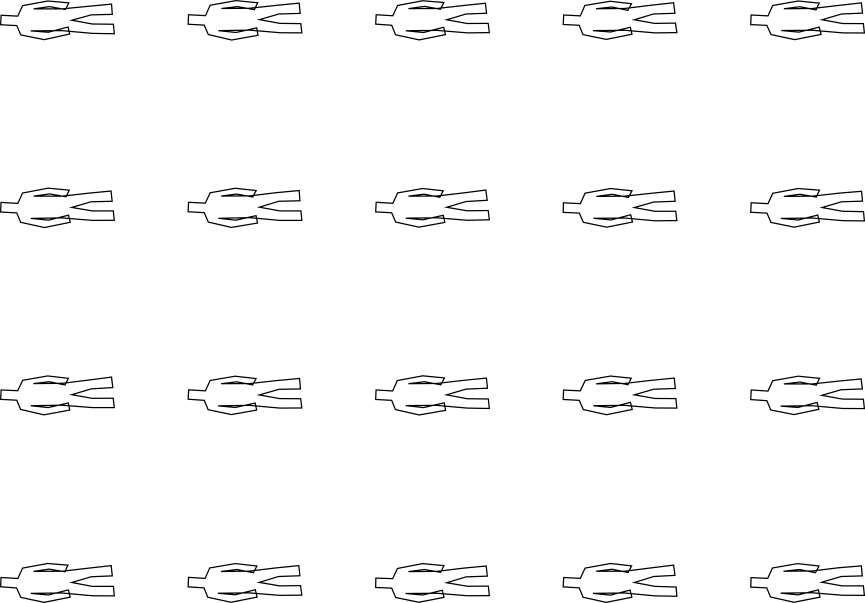
\includegraphics[width=6in]{output/3.learning/correlated_tuning/correlated_tuning_iter0_.png}
\subsubsection{After 10 iterations}

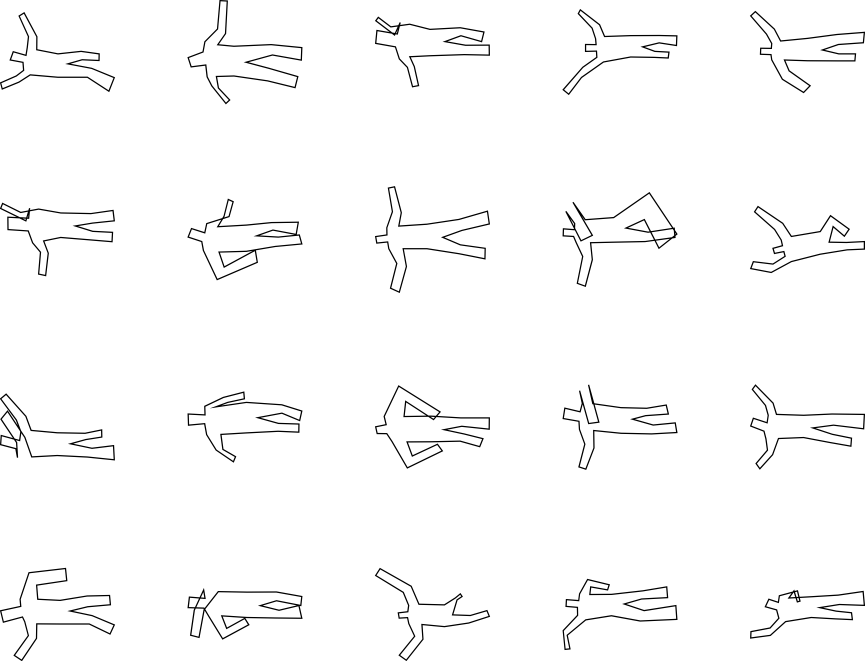
\includegraphics[width=6in]{output/3.learning/correlated_tuning/correlated_tuning_iter10_.png}
\subsubsection{After 20 iterations}

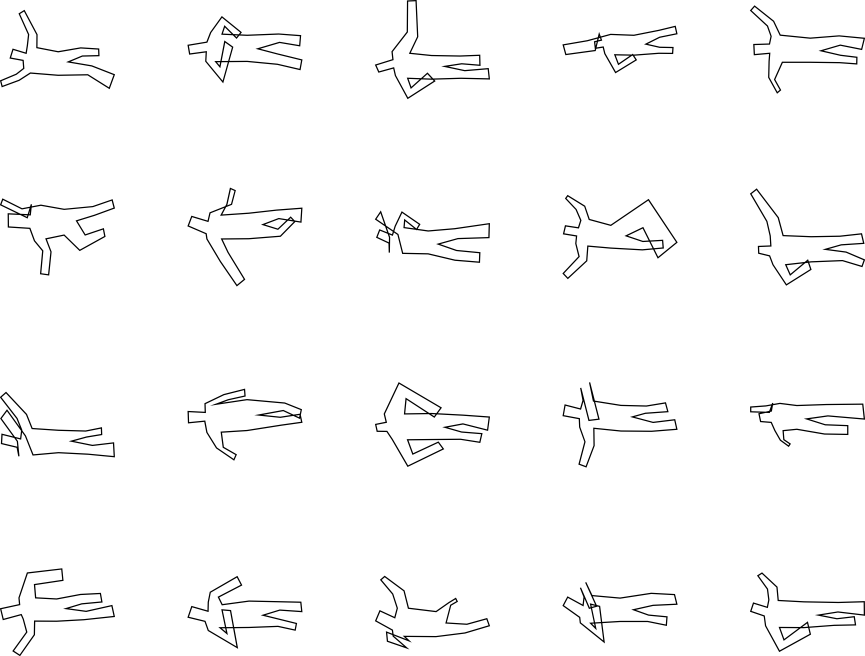
\includegraphics[width=6in]{output/3.learning/correlated_tuning/correlated_tuning_iter20_.png}
\subsubsection{After 30 iterations}

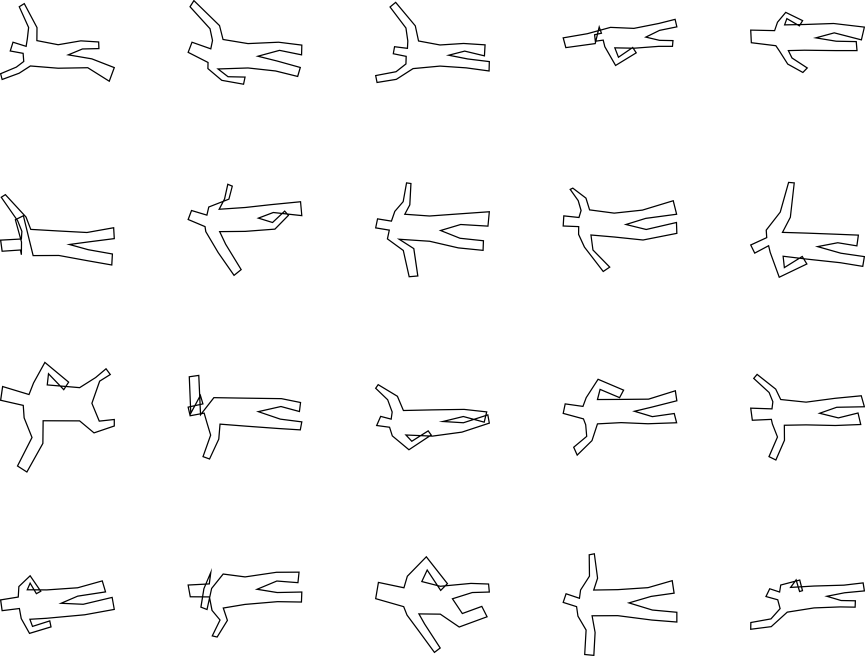
\includegraphics[width=6in]{output/3.learning/correlated_tuning/correlated_tuning_iter30_.png}
\subsection{Correlated tuning with SDF 2}

\subsubsection{After 0 iterations}

\includegraphics[width=6in]{output/3.learning/correlated_tuning/correlated_tuning_iter0_.png}
\subsubsection{After 10 iterations}

\includegraphics[width=6in]{output/3.learning/correlated_tuning/correlated_tuning_iter10_.png}
\subsubsection{After 20 iterations}

\includegraphics[width=6in]{output/3.learning/correlated_tuning/correlated_tuning_iter20_.png}
\subsubsection{After 30 iterations}

\includegraphics[width=6in]{output/3.learning/correlated_tuning/correlated_tuning_iter30_.png}
\subsection{Correlated tuning with SDF 3}

\subsubsection{After 0 iterations}

\includegraphics[width=6in]{output/3.learning/correlated_tuning/correlated_tuning_iter0_.png}
\subsubsection{After 10 iterations}

\includegraphics[width=6in]{output/3.learning/correlated_tuning/correlated_tuning_iter10_.png}
\subsubsection{After 20 iterations}

\includegraphics[width=6in]{output/3.learning/correlated_tuning/correlated_tuning_iter20_.png}
\subsubsection{After 30 iterations}

\includegraphics[width=6in]{output/3.learning/correlated_tuning/correlated_tuning_iter30_.png}


\section{Full Tuning}

In this experiment, we build a grammar from the example curve that
allows all possible decompositions, and then train using EM. Below we
show samples from the grammar after five and ten rounds of
training. Note that there is no longer a choice of initial structure.

\begin{table}\begin{tabular}{|l|l|l|}
\hline
1084815.637311\\
3368.771040\\
2895.491364\\
2780.480195\\
2824.937624\\
2806.935287\\
2806.541103\\
2809.222318\\
2809.821070\\
2809.708171\\
2809.463944\\
2809.102970\\
2808.653905\\
2808.306691\\
2808.177305\\
2808.215122\\
2808.192644\\
2808.174745\\
2808.161250\\
2808.153013\\
2808.150987\\
2808.155995\\
2808.168016\\
2808.184329\\
2808.196037\\
2808.185377\\
2808.134049\\
2808.047173\\
2808.038310\\
2807.843214\\
2807.826409\\
\hline
\end{tabular}\caption{
  Cross-entropy scores across iterations. Each column represents a different starting structure.}\end{table}

\subsection{Tuning with full grammar with SDF 1}

\subsubsection{After 0 iterations}

\includegraphics[width=6in]{output/3.learning/full_tuning/full_tuning_iter0_.png}
\subsubsection{After 10 iterations}

\includegraphics[width=6in]{output/3.learning/full_tuning/full_tuning_iter10_.png}
\subsubsection{After 20 iterations}

\includegraphics[width=6in]{output/3.learning/full_tuning/full_tuning_iter20_.png}
\subsubsection{After 30 iterations}

\includegraphics[width=6in]{output/3.learning/full_tuning/full_tuning_iter30_.png}


% \section{Learning Texture}
% \subsection{Maximum likelihood}
\includegraphics[width=6in]{output/1.models/comparison_gaussians/comparison_gaussians_gaussians_.png}
\subsection{Variance decreased}
\includegraphics[width=6in]{output/1.models/comparison_gaussians/comparison_gaussians_gaussians_decvar_.png}
\subsection{Variance set to zero}
\includegraphics[width=6in]{output/1.models/comparison_gaussians/comparison_gaussians_gaussians_novar_.png}


\section{Learning a model of texture}

\subsection{Class 1}
\includegraphics[width=6in]{output/3.learning/scaled_nts/scaled_nts_1.png}
\subsection{Class 2}
\includegraphics[width=6in]{output/3.learning/scaled_nts/scaled_nts_2.png}
\subsection{Class 3}
\includegraphics[width=6in]{output/3.learning/scaled_nts/scaled_nts_3.png}
\subsection{Class 4}
\includegraphics[width=6in]{output/3.learning/scaled_nts/scaled_nts_4.png}
\subsection{Class 6}
\includegraphics[width=6in]{output/3.learning/scaled_nts/scaled_nts_6.png}
\subsection{Class 7}
\includegraphics[width=6in]{output/3.learning/scaled_nts/scaled_nts_7.png}
\subsection{Class 8}
\includegraphics[width=6in]{output/3.learning/scaled_nts/scaled_nts_8.png}
\subsection{Class 9}
\includegraphics[width=6in]{output/3.learning/scaled_nts/scaled_nts_9.png}
\subsection{Class 12}
\includegraphics[width=6in]{output/3.learning/scaled_nts/scaled_nts_training_12.png}
\includegraphics[width=6in]{output/3.learning/scaled_nts/scaled_nts_12.png}
\subsection{Class 13}
\includegraphics[width=6in]{output/3.learning/scaled_nts/scaled_nts_training_13.png}
\includegraphics[width=6in]{output/3.learning/scaled_nts/scaled_nts_13.png}
\subsection{Class 14}
\includegraphics[width=6in]{output/3.learning/scaled_nts/scaled_nts_training_14.png}
\includegraphics[width=6in]{output/3.learning/scaled_nts/scaled_nts_14.png}
\subsection{Class 15}
\includegraphics[width=6in]{output/3.learning/scaled_nts/scaled_nts_training_15.png}
\includegraphics[width=6in]{output/3.learning/scaled_nts/scaled_nts_15.png}

\end{document}